%%%%%%%%%%%%%%%%%%%%%%%%%%%%%%%%%%%%%%%%%%%%%%%%%%%%%%%%%%%%%%%%%%%%%%%%%%%%%%%

\documentclass[a4paper]{llncs}

%%%%%%%%%%%%%%%%%%%%%%%%%%%%%%%%%%%%%%%%%%%%%%%%%%%%%%%%%%%%%%%%%%%%%%%%%%%%%%%

\usepackage{amsfonts}
\usepackage{amsmath}
\usepackage[all]{xy}
\usepackage{algorithm}
\usepackage[noend]{algpseudocode}



\usepackage{tikz}
\usetikzlibrary{patterns}
\usepackage{subcaption}
\captionsetup{compatibility=false}

%%%%%%%%%%%%%%%%%%%%%%%%%%%%%%%%%%%%%%%%%%%%%%%%%%%%%%%%%%%%%%%%%%%%%%%%%%%%%%%

%%% 
%%% complexity.tex
%%% 

\usepackage{xspace}

%%% ----------------------------------------------------------------------
%%% complexity classes
%%% ----------------------------------------------------------------------

% TIME
\newcommand{\DTIMEX}{{\sf\bf DTIME}}
\newcommand{\DTIMEclass}{\DTIMEX\xspace}
\newcommand{\DTIME}{\DTIMEclass}
% NL class
\newcommand{\NLclassbase}{{\sf\bf NL}}
\newcommand{\NLclass}{\NLclassbase\xspace}
% P class
\newcommand{\Pclassbase}{{\sf\bf P}}
\newcommand{\Pclass}{\Pclassbase\xspace}
% NP class
\newcommand{\NPclassbase}{{\sf\bf NP}}
\newcommand{\NPclass}{\NPclassbase\xspace}
% coNP class
\newcommand{\coNPclassbase}{{\sf\bf coNP}}
\newcommand{\coNPclass}{\coNPclassbase\xspace}
% PSPACE class
\newcommand{\PSPACEclassbase}{{\sf\bf PSPACE}}
\newcommand{\PSPACEclass}{\PSPACEclassbase\xspace}
% MAXSNP class
\newcommand{\MaxSNPclassbase}{{\sf\bf MaxSNP}}
\newcommand{\MaxSNPclass}{\MaxSNPclassbase\xspace}
% MAXNP class
\newcommand{\MaxNPclassbase}{{\sf\bf MaxNP}}
\newcommand{\MaxNPclass}{\MaxNPclassbase\xspace}
% EPTAS class
\newcommand{\EPTASclassbase}{{\sf\bf EPTAS}}
\newcommand{\EPTASclass}{\EPTASclassbase\xspace}
% FPTAS class
\newcommand{\FPTASclassbase}{{\sf\bf FPTAS}}
\newcommand{\FPTASclass}{\FPTASclassbase\xspace}
% PTAS class
\newcommand{\PTASclassbase}{{\sf\bf PTAS}}
\newcommand{\PTASclass}{\PTASclassbase\xspace}
% APX class
\newcommand{\APXclassbase}{{\sf\bf APX}}
\newcommand{\APXclass}{\APXclassbase\xspace}
% log-APX class
\newcommand{\logAPXclassbase}{{\sf\bf log{\tt -}APX}}
\newcommand{\logAPXclass}{\logAPXclassbase\xspace}
% poly-APX class
\newcommand{\polyAPXclassbase}{{\sf\bf poly{\tt -}APX}}
\newcommand{\polyAPXclass}{\polyAPXclassbase\xspace}
% exp-APX class
\newcommand{\expAPXclassbase}{{\sf\bf exp{\tt -}APX}}
\newcommand{\expAPXclass}{\expAPXclassbase\xspace}
% NPO class
\newcommand{\NPOclassbase}{{\sf\bf NPO}}
\newcommand{\NPOclass}{\NPOclassbase\xspace}
% #P class
\newcommand{\sharpPclassbase}{\#{\sf\bf P}}
\newcommand{\sharpPclass}{\sharpPclassbase\xspace}
% FPT class
\newcommand{\FPTclassbase}{{\sf\bf FPT}}
\newcommand{\FPTclass}{\FPTclassbase\xspace}
% W class
\newcommand{\Wclassbase}[1]{{\sf\bf W[#1]}}
\newcommand{\Wclass}[1]{\Wclassbase{#1}\xspace}
% W class
\newcommand{\XPclassbase}{{\sf\bf XP}}
\newcommand{\XPclass}{\XPclassbase\xspace}
% WNL class
\newcommand{\WNLclassbase}{{\sf\bf WNL}}
\newcommand{\WNLclass}{\WNLclassbase\xspace}
% ZPP class
\newcommand{\ZPPclassbase}{{\sf\bf ZPP}}
\newcommand{\ZPPclass}{\ZPPclassbase\xspace}
% NPK class
\newcommand{\NPKclassbase}{{\sf\bf NPK}}
\newcommand{\NPKclass}{\NPKclassbase\xspace}
\newcommand{\NPKandclass}{\text{$\NPKclass_\text{and}$}\xspace}
\newcommand{\NPKzeroandclass}{\text{$\NPKclass^0_\text{and}$}\xspace}
\newcommand{\NPKorclass}{\text{$\NPKclass_\text{or}$}\xspace}
\newcommand{\NPKzeroorclass}{\text{$\NPKclass^0_\text{or}$}\xspace}

%%% ----------------------------------------------------------------------
%%% complete
%%% ----------------------------------------------------------------------

% keyword
\newcommand{\complete}{\text{-complete}}
% NL-complete
\newcommand{\NLcomplete}{\NLclassbase\complete\xspace}
\newcommand{\NLC}{\NLcomplete}
% P-complete
\newcommand{\Pcomplete}{\Pclassbase\complete\xspace}
\newcommand{\PC}{\Pcomplete}
% NP-complete
\newcommand{\NPcomplete}{\NPclassbase\complete\xspace}
\newcommand{\NPC}{\NPcomplete}
% coNP-complete
\newcommand{\coNPcomplete}{\coNPclassbase\complete\xspace}
\newcommand{\coNPC}{\coNPcomplete}
% PSPACE-complete
\newcommand{\PSPACEcomplete}{\PSPACEclassbase\complete\xspace}
\newcommand{\PSPACEC}{\PSPACEcomplete}
% MAXSNP-complete
\newcommand{\MaxSNPcomplete}{\MaxSNPclassbase\complete\xspace}
\newcommand{\MaxSNPC}{\MaxSNPcomplete}
% APX-complete
\newcommand{\APXcomplete}{\APXclassbase\complete\xspace}
\newcommand{\APXC}{\APXcomplete}
% #P-complete
\newcommand{\sharpPcomplete}{\sharpPclassbase\complete\xspace}
\newcommand{\sharpPC}{\sharpPcomplete}
% W[i]-complete
\newcommand{\Wcomplete}[1]{\Wclassbase{#1}\complete\xspace}
\newcommand{\WC}[1]{\Wcomplete{#1}}
% WNL-complete
\newcommand{\WNLcomplete}{\WNLclassbase\complete\xspace}
\newcommand{\WNLC}{\WNLcomplete}

%%% ----------------------------------------------------------------------
%%% hard
%%% ----------------------------------------------------------------------

% keyword
\newcommand{\hard}{\text{-hard}}
% NL-hard
\newcommand{\NLhard}{\NLclassbase\hard\xspace}
\newcommand{\NLH}{\NLhard}
% P-hard
\newcommand{\Phard}{\NPclassbase\hard\xspace}
\newcommand{\PH}{\Phard}
% NP-hard
\newcommand{\NPhard}{\NPclassbase\hard\xspace}
\newcommand{\NPH}{\NPhard}
% coNP-hard
\newcommand{\coNPhard}{\coNPclassbase\hard\xspace}
\newcommand{\coNPH}{\coNPhard}
% PSPACE-hard
\newcommand{\PSPACEhard}{\PSPACEclassbase\hard\xspace}
\newcommand{\PSPACEH}{\PSPACEhard}
% MAXSNP-hard
\newcommand{\MaxSNPhard}{\MaxSNPclassbase\hard\xspace}
\newcommand{\MaxSNPH}{\MaxSNPhard}
% APX-hard
\newcommand{\APXhard}{\APXclassbase\hard\xspace}
\newcommand{\APXH}{\APXhard}
% WNL-hard
\newcommand{\WNLhard}{\WNLclassbase\hard\xspace}
\newcommand{\WNLH}{\WNLhard}
% #P-hard
\newcommand{\sharpPhard}{\sharpPclassbase\hard\xspace}
\newcommand{\sharpPH}{\sharpPhard}
% W[i]-hard
\newcommand{\Whard}[1]{\Wclassbase{#1}\hard\xspace}
\newcommand{\WH}[1]{\Whard{#1}}

%%% ----------------------------------------------------------------------
%%% hardness
%%% ----------------------------------------------------------------------

% keyword
\newcommand{\hardness}{\text{-hardness}}
% NP-hardness
\newcommand{\NPhardness}{\NPclassbase\hardness\xspace}
% APX-hardness
\newcommand{\APXhardness}{\APXclassbase\hardness\xspace}
% W[i]-hardness
\newcommand{\Whardness}[1]{\Wclassbase{#1}\hardness\xspace}
% WNL-hardness
\newcommand{\WNLhardness}{\WNLclassbase\hardness\xspace}

%%% ----------------------------------------------------------------------
%%% completeness
%%% ----------------------------------------------------------------------

% keyword
\newcommand{\completeness}{\text{-completeness}}
% NL-completeness
\newcommand{\NLcompleteness}{\NLclassbase\completeness\xspace}
% P-completeness
\newcommand{\Pcompleteness}{\NPclassbase\completeness\xspace}
% NP-completeness
\newcommand{\NPcompleteness}{\NPclassbase\completeness\xspace}
% APX-completeness
\newcommand{\APXcompleteness}{\APXclassbase\completeness\xspace}
% #P-completeness
\newcommand{\sharpPcompleteness}{\sharpPclassbase\completeness\xspace}
% W[i]-hard
\newcommand{\Wcompleteness}[1]{\W{#1}-\completeness\xspace}

%%% ----------------------------------------------------------------------
%%% reduction
%%% ----------------------------------------------------------------------

\newcommand{\reduction}{reduction}
\newcommand{\reductions}{reductions}
\newcommand{\reductible}{reductible}

\newcommand{\APTypeReduction}{AP}
\newcommand{\PTASTypeReduction}{PTAS}
\newcommand{\LTypeReduction}{L}
\newcommand{\ETypeReduction}{E}
\newcommand{\fptTypeReduction}{fpt}
\newcommand{\pptTypeReduction}{ptp}

% AP-reduction
\newcommand{\APreduction}{\APTypeReduction-\reduction\xspace}
\newcommand{\APreductions}{\APTypeReduction-\reductions\xspace}
\newcommand{\APreductible}{\APTypeReduction-\reductible\xspace}

% PTAS-reduction
\newcommand{\PTASeduction}{\PTASTypeReduction-\reduction\xspace}
\newcommand{\PTASreductions}{\PTASTypeReduction-\reductions\xspace}
\newcommand{\PTASreductible}{\PTASTypeReduction-\reductible\xspace}

% L-reduction
\newcommand{\Lreduction}{\LTypeReduction-\reduction\xspace}
\newcommand{\Lreductions}{\LTypeReduction-\reductions\xspace}
\newcommand{\Lreductible}{\LTypeReduction-\reductible\xspace}

% E-reduction
\newcommand{\Ereduction}{\ETypeReduction-\reduction\xspace}
\newcommand{\Ereductions}{\ETypeReduction-\reductions\xspace}
\newcommand{\Ereductible}{\ETypeReduction-\reductible\xspace}

% fpt-reduction
\newcommand{\fptreduction}{\fptTypeReduction-\reduction\xspace}
\newcommand{\fptreductions}{\fptTypeReduction-\reductions\xspace}
\newcommand{\fptreductible}{\fptTypeReduction-\reductible\xspace}

% ptp-reduction
\newcommand{\ptpreduction}{\ptpTypeReduction-\reduction\xspace}
\newcommand{\ptpreductions}{\ptpTypeReduction-\reductions\xspace}
\newcommand{\ptpreductible}{\ptpTypeReduction-\reductible\xspace}

% symbols
\DeclareMathOperator{\APreduce}{\text{$\leq_{\text{\APTypeReduction}}$}}
\DeclareMathOperator{\PTASreduce}{\text{$\leq_{\text{\PTASTypeReduction}}$}}
\DeclareMathOperator{\Lreduce}{\text{$\leq_{\text{\LTypeReduction}}$}}
\DeclareMathOperator{\Ereduce}{\text{$\leq_{\text{\ETypeReduction}}$}}
\DeclareMathOperator{\fptreduce}{\text{$\leq_{\text{\fptTypeReduction}}$}}
\DeclareMathOperator{\ptpreduce}{\text{$\leq_{\text{\fptTypeReduction}}$}}

%% 
%% Approximation
%%
\DeclareMathOperator{\poly}{poly}
\DeclareMathOperator{\POLY}{poly}
\DeclareMathOperator{\SIZE}{size}
\newcommand{\sol}{{\sf sol}\xspace}
\newcommand{\PB}[1]{\textsf{\scshape{#1}}}
\newcommand{\OPTname}{opt}
\newcommand{\OPT}{\text{$\mathsf{\bf \OPTname}$}}
\newcommand{\OPTpb}[1]{\text{$\mathsf{\OPTname}_{\PB{#1}}$}}
\newcommand{\ALGO}[1]{\text{\small{\ttfamily\sf #1}}}
\newcommand{\Approxname}{Approx}
\newcommand{\APPROX}[1]{\text{$\ALGO{\Approxname}_{\,\PB{#1}}$}}
\newcommand{\PCP}{{\sf\bf PCP}\xspace}

%%
%% Problem Definition
%%
\newcommand{\PbDef}[3]{%
\begin{center}
  \begin{tabular}{l}%
    \shadowbox{%
    \begin{minipage}[c]{.9\textwidth}
      \smallskip%
      \par\noindent%
      {#1}%
      \smallskip
      \par\noindent%
      $\bullet$
      \textbf{\textsf{Input}}~: #2% 
      \medskip
      \par\noindent%
      $\bullet$
      \textbf{\textsf{Question}}~:
      #3% 
      \smallskip%
      \par\noindent%
    \end{minipage}
  }% end shadowbox
  \end{tabular}%
\end{center}
}%
\newcommand{\PbDefinition}{\PbDef}

%%
%% Problem (Input + Output) Definition
%%
\newcommand{\PbInputOutputDef}[3]{%
\begin{center}
  \begin{tabular}{l}%
    \shadowbox{%
    \begin{minipage}[c]{.9\textwidth}
      \smallskip%
      \par\noindent%
      \PB{#1}%
      \medskip%
      \par\noindent%
      $\bullet$
      \textbf{\textsf{Input}}~: #2% 
      \medskip
      \par\noindent%
      $\bullet$
      \textbf{\textsf{Output}}~:
      #3% 
      \smallskip%
      \par\noindent%
    \end{minipage}
  }% end shadowbox
  \end{tabular}%
\end{center}
}%
\newcommand{\PbInputOutputDefinition}{\PbInputOutputDef}


%%
%% Optimization Problem Definition
%%

\newcommand{\OptPbDefinition}[4]{%
\begin{center}
  \begin{tabular}{l}%
    \shadowbox{%
    \begin{minipage}[c]{.9\textwidth}
      \par\noindent%
      \shadowbox{#1}%
      \par\noindent%
      $\bullet$
      \textbf{\textsf{Input}}~: #2% 
      \par\noindent%
      $\bullet$
      \textbf{\textsf{Solution}}~: #3%  
      \par\noindent%
      $\bullet$
      \textbf{\textsf{Measure}}~: #4% 
      \par\noindent%
    \end{minipage}
    }% end shadowbox
  \end{tabular}%
\end{center}
}%

%%
%% Parameterized Problem Definition
%%
\newcommand{\ParamPbDefinition}[4]{%
\begin{center}
  \begin{tabular}{l}%
    %\shadowbox{%
    \begin{minipage}[c]{.95\textwidth}
      % \smallskip%
      \par\noindent%
      #1%
      % \smallskip%
      \par\noindent%
      \textbf{\textsf{Input}}~: #2% 
      % \smallskip
      \par\noindent%
      \textbf{\textsf{Question}}~: #3%  
      % \smallskip
      \par\noindent%
      \textbf{\textsf{Parameter}}~: #4% 
      %\smallskip%
      \par\noindent%
    \end{minipage}
  %}% end shadowbox
  \end{tabular}%
\end{center}
}%
\newcommand{\ParamPbDefinitionTwo}[5]{%
\begin{center}
  \begin{tabular}{l}%
    \shadowbox{%
    \begin{minipage}[c]{.9\textwidth}
      \smallskip%
      \par\noindent%
      \shadowbox{#1}%
      \medskip%
      \par\noindent%
      $\bullet$
      \textbf{\textsf{Input}}~: #2% 
%      \medskip
      \par\noindent%
      $\bullet$
      \textbf{\textsf{Parameter}}~: #3% 
 %     \medskip
      \par\noindent%
      $\bullet$
      \textbf{\textsf{Parameter}}~: #4% 
      \medskip
      \par\noindent%
      $\bullet$
      \textbf{\textsf{Question}}~: #5%  
      \smallskip%
      \par\noindent%
    \end{minipage}
    }% end shadowbox
  \end{tabular}%
\end{center}
}%
\newcommand{\ParamPbDefinitionThree}[6]{%
\begin{center}
  \begin{tabular}{l}%
    \shadowbox{%
    \begin{minipage}[c]{.9\textwidth}
      \smallskip%
      \par\noindent%
      \shadowbox{#1}%
      \medskip%
      \par\noindent%
      $\bullet$
      \textbf{\textsf{Input}}~: #2% 
%      \medskip
      \par\noindent%
      $\bullet$
      \textbf{\textsf{Parameter}}~: #3% 
%      \medskip
      \par\noindent%
      $\bullet$
      \textbf{\textsf{Parameter}}~: #4% 
%      \medskip
      \par\noindent%
      $\bullet$
      \textbf{\textsf{Parameter}}~: #5%  
      \medskip
      \par\noindent%
      $\bullet$
      \textbf{\textsf{Question}}~: #6%  
      \smallskip%
      \par\noindent%
    \end{minipage}
    }% end shadowbox
  \end{tabular}%
\end{center}
}%
\newcommand{\ParamPbDefinitionFour}[7]{%
\begin{center}
  \begin{tabular}{l}%
    \shadowbox{%
    \begin{minipage}[c]{.9\textwidth}
      \smallskip%
      \par\noindent%
      \shadowbox{#1}%
      \medskip%
      \par\noindent%
      $\bullet$
      \textbf{\textsf{Input}}~: #2% 
%      \medskip
      \par\noindent%
      $\bullet$
      \textbf{\textsf{Parameter}}~: #3% 
%      \medskip
      \par\noindent%
      $\bullet$
      \textbf{\textsf{Parameter}}~: #4% 
%      \medskip
      \par\noindent%
      $\bullet$
      \textbf{\textsf{Parameter}}~: #5%  
%      \medskip
      \par\noindent%
    $\bullet$
      \textbf{\textsf{Parameter}}~: #6%  
      \medskip
      \par\noindent%
      $\bullet$
      \textbf{\textsf{Question}}~: #7%  
      \smallskip%
      \par\noindent%
    \end{minipage}
    }% end shadowbox
  \end{tabular}%
\end{center}
}%
\newcommand{\ParamPbDefinitionFive}[8]{%
\begin{center}
  \begin{tabular}{l}%
    \shadowbox{%
    \begin{minipage}[c]{.9\textwidth}
      \smallskip%
      \par\noindent%
      \shadowbox{#1}%
      \medskip%
      \par\noindent%
      $\bullet$
      \textbf{\textsf{Input}}~: #2% 
%      \medskip
      \par\noindent%
      $\bullet$
      \textbf{\textsf{Parameter}}~: #3% 
%      \medskip
      \par\noindent%
      $\bullet$
      \textbf{\textsf{Parameter}}~: #4% 
%      \medskip
      \par\noindent%
      $\bullet$
      \textbf{\textsf{Parameter}}~: #5%  
%      \medskip
      \par\noindent%
    $\bullet$
      \textbf{\textsf{Parameter}}~: #6%  
%      \medskip
      \par\noindent%
    $\bullet$
      \textbf{\textsf{Parameter}}~: #7%  
      \medskip
      \par\noindent%
      $\bullet$
      \textbf{\textsf{Question}}~: #8%  
      \smallskip%
      \par\noindent%
    \end{minipage}
    }% end shadowbox
  \end{tabular}%
\end{center}
}%
\newcommand{\ParamPbDefinitionSix}[9]{%
\begin{center}
  \begin{tabular}{l}%
    \shadowbox{%
    \begin{minipage}[c]{.9\textwidth}
      \smallskip%
      \par\noindent%
      \shadowbox{#1}%
      \medskip%
      \par\noindent%
      $\bullet$
      \textbf{\textsf{Input}}~: #2% 
%      \medskip
      \par\noindent%
      $\bullet$
      \textbf{\textsf{Parameter}}~: #3% 
%      \medskip
      \par\noindent%
      $\bullet$
      \textbf{\textsf{Parameter}}~: #4% 
%      \medskip
      \par\noindent%
      $\bullet$
      \textbf{\textsf{Parameter}}~: #5%  
%      \medskip
      \par\noindent%
      $\bullet$
      \textbf{\textsf{Parameter}}~: #6%  
%      \medskip
      \par\noindent%
      $\bullet$
      \textbf{\textsf{Parameter}}~: #7%  
%      \medskip
      \par\noindent%
      $\bullet$
      \textbf{\textsf{Parameter}}~: #8%  
      \medskip
      \par\noindent%
      $\bullet$
      \textbf{\textsf{Question}}~: #9%  
      \smallskip%
      \par\noindent%
    \end{minipage}
    }% end shadowbox
  \end{tabular}%
\end{center}
}%




%%%%%%%%%%%%%%%%%%%%%%%%%%%%%%%%%%%%%%%%%%%%%%%%%%%%%%%%%%%%%%%%%%%%%%%%%%%%%%%

\DeclareMathOperator{\RUN}{run}
\DeclareMathOperator{\RED}{red}
\DeclareMathOperator{\AV}{Av}

\newcommand{\RLMin}{\text{RLMin}}
\newcommand{\RLMax}{\text{RLMax}}

%%%%%%%%%%%%%%%%%%%%%%%%%%%%%%%%%%%%%%%%%%%%%%%%%%%%%%%%%%%%%%%%%%%%%%%%%%%%%%%

% 231,213
\newcommand{\myPattern}{231,231}

% avoid set
\DeclareMathOperator{\Avd}{Av}
\newcommand\Av[2]{\Avd_{{#1}}({#2})}

% le set de toutes les permitaton
\newcommand{\Perm}[1]{\mathcal{S}_{#1}}

% permutation text
\newcommand{\ptext}{\pi}

\newcommand{\bijection}{B}

% permutation pattern
\newcommand{\ppattern}{\sigma}

\newcommand\BV[2]{\genfrac{}{}{0pt}{}{#1}{#2}}

%Stripe
\DeclareMathOperator{\stripea}{s}
\newcommand{\stripe}[2]{\stripea_{{#1}}[{#2}]}
\newcommand{\stripew}[1]{\stripea_{{#1}}}

% compteur pour les proposition, definition etc...
\newcounter{num}
\setcounter{num}{0}
\newcommand{\num}{\stepcounter{num} }
\newcommand{\numl}[1]{\refstepcounter{num}\label{#1}}

%downstep
\newcommand{\dstep}{d}

%upstep
\newcommand{\ustep}{a}

% MACRO % % % % % % % % % % % % % % % % % % % % % %
\newcommand{\isbelow}{<_y}
\newcommand{\isabove}{>_y}

\newcommand{\ontheleft}{<_x}
\newcommand{\ontheright}{>_x}

\newcommand{\borneinf}{inf}
\newcommand{\bornesup}{sup}

\newcommand{\PM}{PM}


\DeclareMathOperator{\firstia}{first}
\newcommand{\firsti}[2]{\firstia_{{#1}}({#2})}

%\DeclareMathOperator{\run}{run}
\DeclareMathOperator{\block}{block}
\DeclareMathOperator{\LMEi}{LMEp}


\DeclareMathOperator{\factor}{factor}

%first
\DeclareMathOperator{\firsta}{first}
\newcommand{\first}[2]{\firsta(\factor{#1}{#2})}

%binvincular
\newcommand{\x}{X}
\newcommand{\y}{Y}
\newcommand{\bpattern}{(\sigma,\x,\y)}


\newcommand{\sigmaX}{\x_{\sigma}}
\newcommand{\sigmaY}{\y_{\sigma}}

%Pattern Marching
\DeclareMathOperator{\PMa}{PM}
%\newcommand{\PM}[6]{\PMa_{{#1}}^{{#2},{#3},{#4}}({#5},{#6})}

\DeclareMathOperator{\lb}{lb}
\DeclareMathOperator{\ub}{ub}



%LM
\DeclareMathOperator{\LMa}{LM}
\newcommand{\LM}[4]{\LMa_{{#1}}^{{#2}}(#3,#4)}

\DeclareMathOperator{\AFa}{AF}
\newcommand{\AF}[4]{\AFa_{{#1}}^{{#2}}(#3,#4)}

\DeclareMathOperator{\DFa}{DF}
\newcommand{\DF}[4]{\DFa_{{#1}}^{{#2}}(#3,#4)}

%LSC
\DeclareMathOperator{\LCSa}{LCS}
\newcommand{\LCS}[8]{\LCSa_{{#1},{#2},{#3}}^{{#4},{#5},{#6}}({#7},{#8})}

\DeclareMathOperator{\matcha}{M}
\newcommand{\match}[8]{\matcha_{{#1},{#2},{#3}}^{{#4},{#5},{#6}}({#7},{#8})}

%SET OF OCCURENCE
\DeclareMathOperator{\SETa}{S}
\newcommand{\SET}[4]{\SETa_{{#1}}^{{#2}}({#3},{#4})}

%%%%%%%%%%%%%%%%%%%%%%%%%%%%%%%%%%%%%%%%%%%%%%%%%%%%%%%%%%%%%%%%%%%%%%%%%%%%%%%%

\begin{document}

%%%%%%%%%%%%%%%%%%%%%%%%%%%%%%%%%%%%%%%%%%%%%%%%%%%%%%%%%%%%%%%%%%%%%%%%%%%%%%%%

\title{Permutation Pattern matching in\\ $(213,231)$-avoiding permutations}
\author{Both Emerite NEOU, Romeo RIZZI}
\date{}

\author{%
	Both Emerite Neou\thanks{On a Co-tutelle  Agreement with the Department of Mathematics of the University of Trento}\inst{1}
  Romeo Rizzi\inst{2} \and
  St\'ephane Vialette\inst{1}
}% end author
\institute{%
	Universit\'e Paris-Est, LIGM (UMR 8049), CNRS, UPEM, ESIEE Paris, ENPC,
	F-77454, Marne-la-Vallée, France\\
  \email{\{neou,vialette\}@univ-mlv.fr}
  \and
  Department of Computer Science,
  Universit\`a degli Studi di Verona, Italy \\
  \email{romeo.rizzi@univr.it}
}% end institute

\date{\today}

\maketitle

\begin{abstract}
Given permutations $\sigma$ of size $k$ and $\pi$ of size $n$ with $k<n$, the
\emph{permutation pattern matching} problem is to decide whether $\sigma$ occurs
$\pi$ as an order-isomorphic subsequence.
We give a linear-time algorithm in case both $\pi$ and $\sigma$ avoid
the two size-$3$ permutations $213$ and $231$.
For the special case where only $\sigma$ avoids $213$ and $231$, we present a
$O(max(kn^2,n^2\log \log n)$-time algorithm.
We extend our research to bivincular patterns that avoid $213$ and $231$ and present a $O(kn^4)$-time algorithm.
Finally we look at the related problem of the longest subsequence which avoids $213$ and $231$.
\end{abstract}


%%%%%%%%%%%%%%%%%%%%%%%%%%%%%%%%%%%%%%%%%%%%%%%%%%%%%%%%%%%%%%%%%%%%%%%%%%%%%%%%

\section{Introduction}
\label{section:Introduction}



A permutation $\sigma$ is said to \emph{occur} in another permutation $\pi$
(or $\pi$ \emph{contains} $\sigma$),
denoted $\sigma \preceq \pi$,
if there exists a subsequence of elements of $\pi$ that has the same relative
order as $\sigma$.
Otherwise, $\pi$ is said to \emph{avoid} the permutation $\sigma$.
For example a permutation contains the permutation $123$ (resp. $321$) if
it has an increasing (resp. a decreasing) subsequence of size $3$.
Similarly, $213$ occurs in $6152347$, but $231$ does not occurs in $6152347$.
During the last decade, the study of patterns in permutations has
become a very active area of research \cite{Kitaev:book:2011} and
a whole annual conference (\textsc{Permutation Patterns}) focuses
on patterns in permutations.

We consider here the so-called \emph{permutation pattern matching} problem
(also sometimes referred to as the \emph{pattern involvement problem}):
Given two permutations $\sigma$ of size $k$ and $\pi$ of size $n$, the problem is to decide whether
$\sigma \preceq \pi$ (the problem is attributed to Wilf in \cite{Bose:Buss:Lubiw:1998}).
The permutation pattern matching is known to be \NPhard~\cite{Bose:Buss:Lubiw:1998}.
It is however polynomial-time solvable by brute-force enumeration
if $\sigma$ has bounded size.
Improvements to this algorithm were presented in
\cite{Albert:Aldred:Atkinson:Holton:ISAAC:2001} and
\cite{Ahal:Rabinovich:2008},
the latter describing a $O(n^{0.47k+o(k)})$-time algorithm.
Bruner and Lackner \cite{DBLP:journals/corr/abs-1204-5224}
gave a fixed-parameter algorithm solving the permutation pattern matching problem with
an exponential worst-case runtime of $O(1.52^{n}.n.k)$.
This is an improvement upon the $O(k {n \choose k})$ runtime required by
brute-force search without imposing restrictions on $\sigma$ and $\pi$,
where one has to enumerate all the ${n \choose k}$ different subsequences of size $k$ in $\pi$
and test if one of them has the same relative
order as $\sigma$.
Guillemot and Marx \cite{Guillemot:Marx:SODA:2014} showed that the permutation pattern matching problem
is solvable in $2^{O(k^2 \log k)}$, and hence is fixed-parameter tractable with respect to the length $k$
of the pattern $\sigma$ (standard parameterization).
However, Mach proved that the permutation containment problem under the
standard parameterization does not have a polynomial size kernel (assuming $\NPclass \not\subseteq \coNPclass / \POLY$
\cite{Mach:thesis:1992}.

A few particular cases of the permutation pattern matching problem have been attacked successfully.
The case of  increasing patterns is solvable in
$O(n \log \log k)$-time \cite{Crochemore:Porat:2010},
improving the previous 30-year bound of $O(n \log k)$.
% (The algorithm also improves on the previous
% $O(|\pi| \log \log |\pi|)$ bound.)
Furthermore, the patterns $132$, $213$, $231$, $312$ can all be handled in linear-time
by stack sorting algorithms.
Any pattern of size $4$ can be detected in $O(n \log n)$ time
\cite{Albert:Aldred:Atkinson:Holton:ISAAC:2001}.
Algorithmic issues for $321$-avoiding patterns matching for permutations have been investigated in
\cite{Guillemot:Vialette:ISAAC:2009} and more recently in \cite{2015arXiv151006051A}.
The permutation pattern matching problem is also solvable in
polynomial-time for separable patterns \cite{Ibarra:1997,Bose:Buss:Lubiw:1998}
(see also \cite{Bouvel:Rossin:Vialette:CPM:2007} for the longest common subsequence problem and
related ones on separable permutations).
Separable permutations are permutations that do not have an occurrence of
$2413$ nor $3142$, and they are enumerated by the Schr{\"o}der numbers.
%	(sequence A006318 in OEIS).
%	To the best of our knowledge,
%	separable permutations first arose in the work of
%	Avis and Newborn~\cite{Avis:Newborn:1981},
%	who showed that they are precisely the permutations which can be sorted by an
%	arbitrary number of pop-stacks in series,
%	where a pop-stack is a restricted form of stack in which any pop operation
%	pops all items at once.
(Notice that the separable permutations include as a special case the
stack-sortable permutations, which avoid the pattern $231$.)
The major negative result is given in \cite{DBLP:journals/corr/JelinekK16}.
They prove that
the permutation pattern matching problem is \NPC
when $\sigma$ has no decreasing subsequence of length $3$ and
$\pi$ has no decreasing subsequence of length $4$.
This provides the first known example of the permutation pattern matching problem
being hard when one or both of $\pi$ and $\sigma$ are restricted to a proper hereditary
class of permutations.

There exist many generalisations of patterns that are worth considering
in the context of algorithmic issues in pattern matching
(see \cite{Kitaev:book:2011} for an up-to-date survey).
\emph{Vincular patterns}, also called
\emph{generalized patterns},
resemble (classical) patterns with the additional constraint that some of the elements in
a occurrence must be consecutive in positions.
Of particular importance in our context,
Bruner and Lackner \cite{DBLP:journals/corr/abs-1204-5224}
proved that deciding whether a vincular pattern
$\sigma$ of size $k$ occurs in a longer permutation
$\pi$ is $W[1]$-complete for
parameter $k$;
for an up-to-date survey of the $W[1]$ class and related material, see
\cite{Downey:Fellows:2013}.
\emph{Bivincular patterns} generalize classical patterns even further
than vincular
patterns by adding a constraint on values.

We focus in this paper on pattern matching issues for \emph{wedge permutations}
(\emph{i.e.}, those permutations that avoid both $213$ and $231$). 
%The number of $n$-wedge permutations is
%$t_0 = 1$ for $n = 0$ and
%$t_n =2^{n-1}$ for $n\geq 1$ \cite{Simion:Schmidt:EJC:1985},
%as they are in bijection with binary word of size $n-1$.
%On an individual basis,
%the permutations that do not have an occurrence of the permutation pattern $231$
%are exactly the \emph{stack-sortable permutations} and they are counted by
%the Catalan numbers \cite{Knuth:1997:ACP:260999}.
%	A stack-sortable permutation is a permutation whose elements may be sorted by
%	an algorithm whose internal storage is limited to a single stack data structure.
%	As for $213$, it is well-known that
% 	if $\pi = \pi_1\pi\,\ldots\,\pi_n$ avoids $132$, then its complement
% 	$\pi' = (n+1-\pi_1)(n+1-\pi_2)\,\ldots\,(n+1-\pi_n)$ avoids $312$, and
% 	the reverse of $\pi'$ avoids $213$.
% From a combinatorial point of view,
% B\'ona \cite{Bona:ElJC:2012}
% showed the rather surprising fact that the cumulative number of
% occurrences of the classical patterns $231$ and $213$ are the same on the
% set of permutations avoiding $132$,
% beside the pattern based statistics $231$ and $213$
% do not have the same distribution on this set.
% \emph{Almost avoidance} has also been considered;
% a permutation $\pi$ almost avoids a set $X$ of permutations
% if there is a way to remove a single element of $\pi$ to get a permutation
% that avoids all elements in $P$
% and $L_n(P)$ denotes the set of permutations of length $n$ that almost avoid
% $P$.
% It is shown in \cite{Griffiths:Smith:Warren:PMA:2011} that
% $L_n(213, 231) = L_n(132, 231) = L_n(132, 312) = L_n(213, 312)$.
This paper is organized as follows.
In Section~\ref{section:Definitions} the needed definitions are presented.
Section~\ref{section:both are (213,231)-avoiding} is devoted to presenting
an online linear-time algorithm in case both
permutations are wedge permutations,
whereas Section~\ref{section:sigma only avoid 231 and 213} focuses on the case
where only the pattern is a wedge permutation.
In Section~\ref{section:bivincular} we give a polynomial-time algorithm
for a bivincular wedge permutation pattern.
In Section~\ref{section:LCS} we consider the problem of finding the longest
wedge permutation pattern in permutations.


%%%%%%%%%%%%%%%%%%%%%%%%%%%%%%%%%%%%%%%%%%%%%%%%%%%%%%%%%%%%%%%%%%%%%%%%%%%%%%%%

\section{Definitions}
\label{section:Definitions}

A \textit{permutation} of size $n$ is a linear ordering of an ordered set of size $n$.
When writing the permutation we omit the $<$ sign, thus
writing the permutation as a word:
$\pi = \pi_1\pi_2\,\ldots\,\pi_n$, whose elements are distinct
and usually consist of the integers $1,2,\ldots,n$.

We need to consider both the natural order of the set
and the linear order given by the permutation.
When talking about an element,
we refer to the relative position in
the natural order of the set
as its value
and
we refer to the relative position
in the order given by the permutation
as its position.
We write
$\pi[i]$ to indicate the value of the element
at position $i$ (\emph{i.e.} $\pi_i$).
For example, in the permutation $\pi = 51342$,
The element $1$ is at position $2$
and the element at position $1$ has for value $5$.
Conveniently, we let
$\pi[i:j]$ stand for
$\pi_i\pi_{i+1}\,\ldots\,\pi_j$,
$\pi[:j]$ stand for $\pi[1:j]$ and
$\pi[i:]$ stand for $\pi[i:n]$.

It is convenient to use a geometric representation of permutations
to ease the understanding of algorithms.
The geometric representation corresponds to the set of points with coordinate $(i,\pi[i])$
(see Figure \ref{example: pattern matching}).


When an element $\pi[\alpha]$ is smaller (resp. larger)
than an element $\pi[\beta]$  by value (in the natural order of the set),
we say that $\pi[\alpha]$ is below (resp. above) $\pi[\beta]$,
as a reference to the geometric representation of the permutation.
Besides, the element with the largest value is called
the topmost element and the element with the smallest value
is called the bottommost element.
For example, in the permutation $\pi = 51342$,
$2$ is below $4$, the topmost element is $5$
and the bottommost element is $1$.

When an element $\pi[\alpha]$ is smaller (resp. larger)
than an element $\pi[\beta]$  by position (in the order given by the permutation),
we say that $\pi[\alpha]$ is on the left of (resp. on the right of) $\pi[\beta]$.
Besides, the element with the largest position is called the rightmost element
and the element with the smallest position is called the leftmost element.
For example, in the permutation $\pi = 51342$,
$5$ is on the left of $3$, the leftmost element is $5$
and the rightmost element is $2$.


% The \emph{reduced form} of a permutation $\sigma$ on a set
% $\{j_1, j_2, \ldots, j_k\}$ where
% $j_1 < j_2 < \ldots < j_n$ is the permutation $\sigma'$
% obtained by renaming the letters of $\sigma$ so that
% $j_i$ is renamed $i$ for all $1 \leq i \leq k$.
% We let $\RED(\sigma)$ denote the reduced form of $\sigma$.
% For example $\RED(453) = 231$
% while $\RED(3174) = 2143$.

A permutation $\sigma$ is said to \emph{occur} in the permutation $\pi$, written $\sigma \preceq \pi$,
if there exists a subsequence of (not necessarily consecutive)
elements of $\pi$ that has the same relative order as $\sigma$.
Such subsequence is called an \emph{occurrence} of $\sigma$ in $\pi$.
Otherwise, $\pi$ is said to \emph{avoid} the permutation $\sigma$.
For example, the permutation $\pi = 391867452$
has an occurrence of the pattern $\sigma = 51342$,
as can be seen in the highlighted subsequence of
$\pi = 3\mathbf{9}\mathbf{1}8\mathbf{6}\mathbf{7}\mathbf{4}52$
(or
$\pi = 3\mathbf{9}\mathbf{1}8\mathbf{6}\mathbf{7}4\mathbf{5}2$
or
$\pi = 3\mathbf{9}\mathbf{1}8\mathbf{6}\mathbf{7}45\textbf{2}$
or
$\pi = 3\mathbf{9}\mathbf{1}867\textbf{4}\textbf{5}\mathbf{2}$
).
Since the permutation $\pi = 391867452$  contains no increasing subsequence of
size four, $\pi$ avoids $1234$.

For an occurrence $s$ of $\sigma$ in $\pi$,
we say that $\pi[j]$ correspond $\sigma[i]$ in the occurrence or
that $\sigma[i]$ is matched to $\pi[j]$  in the occurrence
if and only if $\pi[j]=s[i]$.
Geometrically, $\pi$ has an occurrence of $\sigma$ if there exists
a set of points in $\pi$ whose relative positions are the same as those of $\sigma$
(see Figure \ref{example: pattern matching}).
%% In other words,
%% if there exists a set of points in $\pi$ with the same disposition as the set of points of $\sigma$,
%% regardless of the distance (see Figure \ref{example: pattern matching}).

\begin{figure}
	\centering
		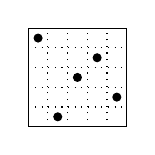
\begin{tikzpicture}[scale=.25]
		\draw (0,0) -- (5,0) -- (5,5) -- (0,5) -- cycle;
		\foreach \i in {1, 2, 3, 4, 5}{
			\draw[dotted] (0,\i) -- (5, \i);
			\draw[dotted] (\i,0) -- (\i, 5);
		}
		\draw[fill=black] (0.5,4.5) circle (2mm);
		\draw[fill=black] (1.5,0.5) circle (2mm);
		\draw[fill=black] (2.5,2.5) circle (2mm);
		\draw[fill=black] (3.5,3.5) circle (2mm);
		\draw[fill=black] (4.5,1.5) circle (2mm);
		\end{tikzpicture}
		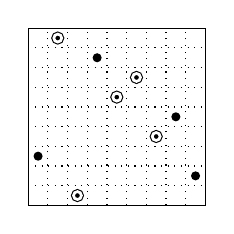
\begin{tikzpicture}[scale=.25]
		\draw (0,0) -- (9,0) -- (9,9) -- (0,9) -- cycle;
		\foreach \i in {1, 2, 3, 4, 5, 6, 7, 8, 9}{
			\draw[dotted] (0,\i) -- (9, \i);
			\draw[dotted] (\i,0) -- (\i, 9);
		}
		\draw[fill=black] (0.5,2.5) circle (2mm);
		\draw[fill=black,double, double distance=1pt] (1.5,8.5) circle (2mm);
		\draw[fill=black,double, double distance=1pt] (2.5,0.5) circle (2mm);
		\draw[fill=black] (3.5,7.5) circle (2mm);
		\draw[fill=black,double, double distance=1pt] (4.5,5.5) circle (2mm);
		\draw[fill=black,double, double distance=1pt] (5.5,6.5) circle (2mm);
		\draw[fill=black,double, double distance=1pt] (6.5,3.5) circle (2mm);
		\draw[fill=black] (7.5,4.5) circle (2mm);
		\draw[fill=black] (8.5,1.5) circle (2mm);
		\end{tikzpicture}
		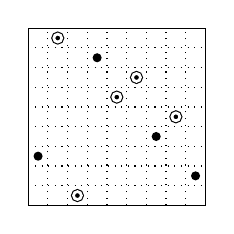
\begin{tikzpicture}[scale=.25]
		\draw (0,0) -- (9,0) -- (9,9) -- (0,9) -- cycle;
		\foreach \i in {1, 2, 3, 4, 5, 6, 7, 8, 9}{
			\draw[dotted] (0,\i) -- (9, \i);
			\draw[dotted] (\i,0) -- (\i, 9);
		}
		\draw[fill=black] (0.5,2.5) circle (2mm);
		\draw[fill=black,double, double distance=1pt] (1.5,8.5) circle (2mm);
		\draw[fill=black,double, double distance=1pt] (2.5,0.5) circle (2mm);
		\draw[fill=black] (3.5,7.5) circle (2mm);
		\draw[fill=black,double, double distance=1pt] (4.5,5.5) circle (2mm);
		\draw[fill=black,double, double distance=1pt] (5.5,6.5) circle (2mm);
		\draw[fill=black] (6.5,3.5) circle (2mm);
		\draw[fill=black,double, double distance=1pt] (7.5,4.5) circle (2mm);
		\draw[fill=black] (8.5,1.5) circle (2mm);
		\end{tikzpicture}
		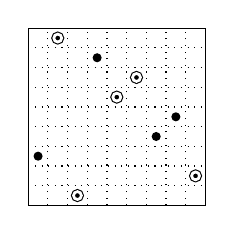
\begin{tikzpicture}[scale=.25]
		\draw (0,0) -- (9,0) -- (9,9) -- (0,9) -- cycle;
		\foreach \i in {1, 2, 3, 4, 5, 6, 7, 8, 9}{
			\draw[dotted] (0,\i) -- (9, \i);
			\draw[dotted] (\i,0) -- (\i, 9);
		}
		\draw[fill=black] (0.5,2.5) circle (2mm);
		\draw[fill=black,double, double distance=1pt] (1.5,8.5) circle (2mm);
		\draw[fill=black,double, double distance=1pt] (2.5,0.5) circle (2mm);
		\draw[fill=black] (3.5,7.5) circle (2mm);
		\draw[fill=black,double, double distance=1pt] (4.5,5.5) circle (2mm);
		\draw[fill=black,double, double distance=1pt] (5.5,6.5) circle (2mm);
		\draw[fill=black] (6.5,3.5) circle (2mm);
		\draw[fill=black] (7.5,4.5) circle (2mm);
		\draw[fill=black,double, double distance=1pt] (8.5,1.5) circle (2mm);
		\end{tikzpicture}
		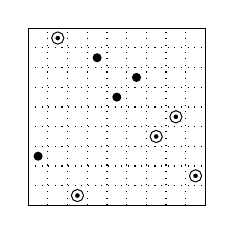
\begin{tikzpicture}[scale=.25]
		\draw (0,0) -- (9,0) -- (9,9) -- (0,9) -- cycle;
		\foreach \i in {1, 2, 3, 4, 5, 6, 7, 8, 9}{
			\draw[dotted] (0,\i) -- (9, \i);
			\draw[dotted] (\i,0) -- (\i, 9);
		}
		\draw[fill=black] (0.5,2.5) circle (2mm);
		\draw[fill=black,double, double distance=1pt] (1.5,8.5) circle (2mm);
		\draw[fill=black,double, double distance=1pt] (2.5,0.5) circle (2mm);
		\draw[fill=black] (3.5,7.5) circle (2mm);
		\draw[fill=black] (4.5,5.5) circle (2mm);
		\draw[fill=black] (5.5,6.5) circle (2mm);
		\draw[fill=black,double, double distance=1pt] (6.5,3.5) circle (2mm);
		\draw[fill=black,double, double distance=1pt] (7.5,4.5) circle (2mm);
		\draw[fill=black,double, double distance=1pt] (8.5,1.5) circle (2mm);
		\end{tikzpicture}




	\caption[Example pattern matching]{
		The pattern $\sigma=51342$
		and four occurrences of $\sigma$ in $391867452$.}
	\label{example: pattern matching}
\end{figure}

%Suppose $P$ is a set of permutations. We let $\AV_n(P)$ denote the
%set of all $n$-permutations avoiding each permutation in $P$.
%For the sake of convenience
%(and as it is customary~\cite{Kitaev:book:2011}), we omit $P$'s braces thus having
%e.g. $\AV_n(213,231)$ instead of
%$\AV_n(\{213,231\})$.
%If $\pi \in \AV_n(P)$, we also say that $\pi$ is
%\emph{$P$-avoiding}.

% A basic example is if
% $\pi = \pi_1\pi_2\,\ldots\,\pi_n \in \AV_n(321)$, i.e.,
% has no decreasing subsequence of length $3$, then its reverse,
% $\pi' = \pi_n\pi_{n-1}\,\ldots\,\pi_1$ avoids $123$, i.e.,
% has no increasing subsequence of length $3$.

%An \emph{ascent element} of an $n$-permutation $\pi \in S_n$ is any element
%$\pi[i]$ such that $i<n$ and $\pi[i] < \pi[i+1]$.
%For example, the permutation
%$3452167$ has ascents $3$, $4$, $1$ and $6$.
%Similarly, a \emph{descent} is any element
%$\pi[i]$ such that $i<n$ and $\pi[i] > \pi[i+1]$.
%So for every $1 \leq i < n$, $\pi[i]$  is either an ascent or a descent of
%$\pi$.

%To clarify the exposition,
%we let $\ustep$ and $\dstep$ denote an ascend and a descend, resp..
%The \emph{stripe} $s_\pi$ of a permutation $\pi \in S_n$ is the word
%$\stripe{\pi}{1} \stripe{\pi}{2} \ldots \stripe{\pi}{n-1} \in \{\ustep,\dstep\}^{n-1}$
%defined by
%$\stripe{\pi}{i}= \ustep$ if $i$ an ascent in $\pi$ and
%$\stripe{\pi}{i} = \dstep$ if $i$ a descent in $\pi$.
%For example the stripe of the permutation
%$\pi = 981234765$
%is $\stripew{\pi} = \dstep\dstep\ustep\ustep\ustep\ustep\dstep\dstep$.

A $\textit{right-to-left maximum}$ (\RLMax, for short) of $\pi$ is an element that does not have any element above it and to its right (see Figure $\ref{fig:left to right maxima}$). Formally, $\pi[i]$ is a \RLMax if and only if $\pi[i]$ is topmost element of $\pi[i:]$. Similarly $\pi[i]$ is a $\textit{right-to-left minimum}$ (\RLMin, for short) if and only if $\pi[i]$ is the bottommost element of $\pi[i:]$.

\begin{figure}
	\centering
	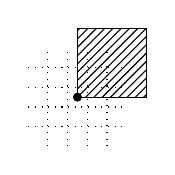
\begin{tikzpicture}[scale=.25]
	\foreach \i in {1, 2, 3, 4}{
		\draw[dotted] (0,\i) -- (5, \i);
		\draw[dotted] (\i,0) -- (\i, 5);
	}
	\draw[fill=black] (2.5,2.5) circle (2mm);
	%\draw (2.5,2.5) -- (2.5,6.5);
	%\draw (2.5,2.5) -- (6,2.5);

	\draw [pattern=north east lines] (2.5,2.5) rectangle (6,6);

	\end{tikzpicture}





	\caption[Example pattern matching]{
		The element is a \RLMax if and only if the hashed area is empty.}
	\label{fig:left to right maxima}
\end{figure}

A \emph{bivincular permutation pattern} $\widetilde{\sigma}$
of size $k$ is a permutation written in
two-line notation
(the top row is $12\,\ldots\,k$ and the bottom row
is a permutation $\sigma_1\sigma_2\,\ldots\,\sigma_k$)
with overlined elements in the top row and underlined elements in the bottom row.
We have the following conditions on the top and bottom rows
of $\sigma$, as seen in \cite{Kitaev:book:2011} in Definition 1.4.1:
\begin{itemize}
	\item
	If the bottom line of $\sigma$ contains
	$\underline{\sigma_i\sigma_{i+1}\,\ldots\,\sigma_j}$
	then the elements corresponding to
	$\sigma_i\sigma_{i+1}\,\ldots\,\sigma_j$ in a occurrence of
	$\sigma$ in $\pi$ must be adjacent, whereas there is
	no adjacency condition for
	non-underlined consecutive elements.
	Moreover if the bottom row of $\sigma$ begins with
	$_\llcorner{\sigma_1}$ then any occurrence of $\sigma$
	in a permutation $\pi$ must begin with the leftmost
	element of $\pi$,
	and
	if the bottom row of $\sigma$ ends with
	${\sigma_k}_\lrcorner$ then any occurrence of $\sigma$
	in a permutation $\pi$ must end with the rightmost
	element of $\pi$.
	\item
	If the top line of $\sigma$ contains
	$\overline{i\,i+1\,\ldots\,j}$ then the elements corresponding to
	$i, i+1, \ldots, j$ in an
	occurrence of $\sigma$ in $\pi$ must be adjacent in values,
	whereas there is no value adjacency restriction for non-overlined
	elements.
	Moreover, if the top row of $\sigma$ begins with
	$^\ulcorner{1}$ then
	any occurrence of $\sigma$ in a permutation $\pi$ must contain
	the bottommost element of $\pi$, and
	if top row of $\sigma$ ends with $k^\urcorner$ then
	any occurrence of $\sigma$ in a permutation $\pi$ must contain
	the topmost element of $\pi$.
\end{itemize}

Given a bivincular permutation pattern $\widetilde{\sigma}$,
$\sigma$ refers to the bottom line of $\widetilde{\sigma}$
without any element underlined.
For example,
let
$\widetilde{\sigma} = \BV{1\overline{23}4\urcorner}{\llcorner 21\underline{43}}$,
in $3217845$, $\textbf{32}17\textbf{84}5$ is an occurrence  of $\widetilde{\sigma}$ but $3\textbf{21}\textbf{7}8\textbf{4}5$ is not
and $\sigma = 2143$.
The best general reference for bivincular pattern is \cite{Kitaev:book:2011}.





Geometrically, we represent underlined and overlined elements by \textit{forbidden areas}.
If two elements are overlined then we draw a horizontal forbidden area between those two points.
In an occurrence, we also draw the forbidden area between the matching of two overlined elements.
This area must be empty to have a valid occurrence of the bivincular pattern.
If the area is empty then there is no element between them when reading the permutation
from bottom to top,
in other words the matching elements are consecutive in value.
If two elements are underlined then we draw a vertical forbidden area.
(See Figure \ref{example:bivincular pattern matching}).


\begin{figure}[t]
	\centering

    	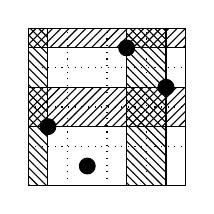
\begin{tikzpicture}[scale=.5]
    	\draw [pattern=north east lines] (0,1.5) rectangle (4,2.5);
    	\draw [pattern=north east lines] (0,3.5) rectangle (4,4);

    	\draw [pattern=north west lines] (0,0) rectangle (0.5,4);
    	\draw [pattern=north west lines] (2.5,0) rectangle (3.5,4);


    	\draw (0,0) -- (4,0) -- (4,4) -- (0,4) -- cycle;
    	\foreach \i in {1, 2, 3, 4}{
    		\draw[dotted] (0,\i) -- (4, \i);
    		\draw[dotted] (\i,0) -- (\i, 4);
    	}
    	\draw[fill=black] (0.5,1.5) circle (2mm);
    	\draw[fill=black] (1.5,0.5) circle (2mm);
    	\draw[fill=black] (2.5,3.5) circle (2mm);
    	\draw[fill=black] (3.5,2.5) circle (2mm);
    	\end{tikzpicture}
    	\quad
    	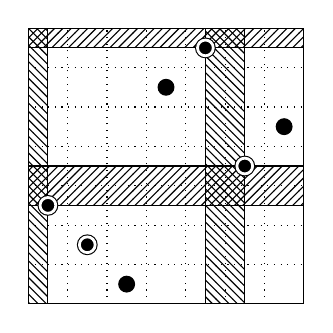
\begin{tikzpicture}[scale=.5]
    	\draw [pattern=north east lines] (0,6.5) rectangle (7,7);
    	\draw [pattern=north east lines] (0,2.5) rectangle (7,3.5);

    	\draw [pattern=north west lines] (0,0) rectangle (0.5,7);
    	\draw [pattern=north west lines] (4.5,0) rectangle (5.5,7);

    	%$3217845$

    	\draw (0,0) -- (7,0) -- (7,7) -- (0,7) -- cycle;
    	\foreach \i in {1, 2, 3, 4, 5, 6, 7}{
    		\draw[dotted] (0,\i) -- (7, \i);
    		\draw[dotted] (\i,0) -- (\i, 7);
    	}

		\draw[fill=black,double, double distance=1pt] (0.5,2.5) circle (2mm);
		\draw[fill=black,double, double distance=1pt] (1.5,1.5) circle (2mm);
		\draw[fill=black] (2.5,0.5) circle (2mm);
		\draw[fill=black] (3.5,5.5) circle (2mm);
		\draw[fill=black,double, double distance=1pt] (4.5,6.5) circle (2mm);
		\draw[fill=black,double, double distance=1pt] (5.5,3.5) circle (2mm);
		\draw[fill=black] (6.5,4.5) circle (2mm);

    	\end{tikzpicture}
    	\quad
    	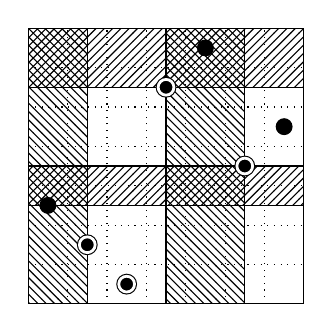
\begin{tikzpicture}[scale=.5]
    	\draw [pattern=north east lines] (0,5.5) rectangle (7,7);
    	\draw [pattern=north east lines] (0,2.5) rectangle (7,3.5);

    	\draw [pattern=north west lines] (0,0) rectangle (1.5,7);
    	\draw [pattern=north west lines] (3.5,0) rectangle (5.5,7);

    	%$3217845$

    	\draw (0,0) -- (7,0) -- (7,7) -- (0,7) -- cycle;
    	\foreach \i in {1, 2, 3, 4, 5, 6, 7}{
    		\draw[dotted] (0,\i) -- (7, \i);
    		\draw[dotted] (\i,0) -- (\i, 7);
    	}

    	\draw[fill=black] (0.5,2.5) circle (2mm);
    	\draw[fill=black,double, double distance=1pt] (1.5,1.5) circle (2mm);
    	\draw[fill=black,double, double distance=1pt] (2.5,0.5) circle (2mm);
    	\draw[fill=black,double, double distance=1pt] (3.5,5.5) circle (2mm);
    	\draw[fill=black] (4.5,6.5) circle (2mm);
    	\draw[fill=black,double, double distance=1pt] (5.5,3.5) circle (2mm);
    	\draw[fill=black] (6.5,4.5) circle (2mm);

    	\end{tikzpicture}



    	\caption[Example pattern matching]{
    		From left to right,
    		the bivincular pattern $\widetilde{\sigma} = \BV{1\overline{23}4\urcorner}{\llcorner 21\underline{43}  }$, an occurrence of $\widetilde{\sigma}$ in $3216745$, an occurrence of $\sigma$ in $3216745$ but not an occurrence of $\widetilde{\sigma}$ because the points $(1,3)$ and $(5,7)$ are in the forbidden areas.}
    	\label{example:bivincular pattern matching}
\end{figure}

%%%%%%%%%%%%%%%%%%%%%%%%%%%%%%%%%%%%%%%%%%%%%%%%%%%%%%%%%%%%%%%%%%%%%%%%%%%%%%%%

\section{Both $\pi$ and $\sigma$ are wedge permutation}
\label{section:both are (213,231)-avoiding}



This section is devoted to present a fast algorithm for deciding if
$\sigma \preceq \pi$
in case both $\pi$ and $\sigma$ are wedge permutations.
We begin with an easy and folk  but crucial structure lemma.

\begin{lemma} %[Folklore]
\label{lemma:first element is 1 or n}
The first element of any wedge permutations
must be either the bottommost or the topmost element.
\end{lemma}

\begin{proof} %[of Lemma~\ref{lemma:first element is 1 or n}]
Any other initial element would serve as a `$2$' in either a
$231$ or $213$ with $1$ and $n$ as the `$1$' and `$3$' resp..
\qed
\end{proof}


\begin{corollary}
\label{corollary:minmaxelement}
$\pi$ is a wedge permutation of size $n$ if and only if for $1 \leq i \leq n$,
$\pi[i]$ is a \RLMax or a \RLMin.
\end{corollary}

%% \begin{proof} %[of Lemma~\ref{lemma:first element is 1 or n}]
%% Given a position $i$, $\pi[i:]$ is a wedge permutation,
%% so it either starts with the maximal or the minimal element.
%% \qed
%% \end{proof}

As a consequence, every element of a wedge permutation can be partitioned
into three sets: the set of \RLMax elements, the set of \RLMin elements and the
rightmost element which can be both a \RLMax element and a \RLMin element.

\begin{remark}
The set of \RLMax elements is a decreasing subsequence,
indeed each element is left above the next \RLMax element by definition
of a \RLMax element. In the same fashion,
the set of \RLMin elements is an increasing subsequence.
See Figure~\ref{fig:shape of the permutation plus factor}.
\end{remark}

\begin{remark}
Every element of the set of \RLMax elements is above the elements
of the set of the \RLMin elements.
In other words, a wedge permutations
can be cut in half horizontally on the rightmost element such that the upper half contains a decreasing
subsequence and the lower half contains an increasing subsequence.
This shape the permutation as a $>$,
hence the name of wedge permutations.
See Figure~\ref{fig:shape of the permutation plus factor}.
\end{remark}

\begin{remark}
The partition gives a bijection between the set of wedge permutations of size $n$ where the elements are $1,\ldots,n$
and the set of binary word of size $n-1$.
The word $w$ which corresponds to $\pi$ is the word where each letter at position $i$
represents whether $\pi[i]$ is a \RLMax element or a \RLMin element.
We call this bijection $\bijection$.
\end{remark}

To figure out whether or not an element is a \RLMax element or a \RLMin element,
one has to run the whole permutation from left to right starting
from the position of the element, we give a corollary of lemma~\ref{lemma:first element is 1 or n}, to guest it in constant time.

\begin{corollary}
\label{corollary:max is ascent}
Let $\pi$ be a wedge permutation and $1 \leq i < n$. Then,
\begin{enumerate}
\item $\pi[i]$ is a \RLMin element if and only if $\pi[i]<\pi[i+1]$
\item $\pi[i]$ is a \RLMax element if and only if $\pi[i]>\pi[i+1]$ is a \RLMax
\end{enumerate}

\end{corollary}

%\begin{remark}
%Corollary~\ref{corollary:max is ascent} allows to compute
%\end{remark}

%For convenience when drawing a random wedge permutation
%we will sometime represent a sequence of ascent/descent element by lines (see Figure \ref{fig:shape of the permutation} and \ref{fig:shape of the permutation plus factor}).


%\begin{figure}[t]
%	\centering
%	\begin{tikzpicture}[scale=.3]
%	\draw (0,0) -- (9,0) -- (9,9) -- (0,9) -- cycle;
%	\foreach \i in {1, 2, 3, 4, 5, 6, 7, 8, 9}{
%		\draw[dotted] (0,\i) -- (9, \i);
%		\draw[dotted] (\i,0) -- (\i, 9);
%	}
%	\draw[fill=black] (0.5,0.5) circle (2mm);
%	\draw[fill=black] (1.5,1.5) circle (2mm);
%	\draw[fill=black] (2.5,2.5) circle (2mm);
%	\draw[fill=black] (3.5,8.5) circle (2mm);
%	\draw[fill=black] (4.5,7.5) circle (2mm);
%	\draw[fill=black] (5.5,3.5) circle (2mm);
%	\draw[fill=black] (6.5,6.5) circle (2mm);
%	\draw[fill=black] (7.5,5.5) circle (2mm);
%	\draw[fill=black] (8.5,4.5) circle (2mm);
%
%	\draw (0,0) -- (3,3);
%	\draw (3,9) -- (5,7);
%	\draw (5,3) -- (6,4);
%	\draw (6,7) -- (9,4);
%
%
%	\end{tikzpicture}
%
%
%	\caption{The wedge permutation $123984765$, every point which is on a north-west to south-east line represents a descent element and every point which is on a south-west to north-east line represents an ascent element.}
%	\label{fig:shape of the permutation}
%\end{figure}

Now that we had highlight some structural point of a wedge permutation,
we can use this structure to solve the permutation pattern matching.
More precisely, we use the bijection on binary word to solve this problem,
thank to the following lemma.

\begin{lemma}
\label{lemma:MatchStripeToPermutation}
Let $\pi$ and $\sigma$ be two wedge permutations.
Then, $\pi$ has an occurrence of $\sigma$ if and only if
there exists a subsequence $t$ of $\pi$ such $\bijection(t)=\bijection(\sigma)$.
\end{lemma}

\begin{proof} %[of Lemma~\ref{lemma:MatchStripeToPermutation}]
The forward direction is obvious.
We prove the backward direction by induction on the size of
$\sigma$: if $\bijection(t)=\bijection(\sigma)$ then $t$ is an occurrence of $\sigma$.
The base case is a pattern of size $2$.
Suppose that $\sigma = 12$ and thus $\bijection(\sigma) = \RLMin$.
Let $t = \pi_{i_1}\pi_{i_2}$, $i_1 < i_2$, be a subsequence of $\pi$
such that $\bijection(t) = \RLMin$, this reduces to saying that
$\pi_{i_1} < \pi_{i_2}$,
and hence that $t$ is an occurrence of $\sigma = 12$ in $\pi$.
A similar argument shows that the lemma holds for $\sigma = 21$.
Now, assume that the lemma is true for all patterns up to size $k \geq 2$.
Let $\sigma$ be a wedge permutation of size $k+1$ and
let $t$
be a subsequence of $\pi$ of size $k+1$ such that
$\bijection(t) = \bijection(\sigma)$.
As $\bijection(t)[2:] = \bijection(\sigma)[2:]$
by the induction hypothesis, it follows that
$t[2:]$ is an occurrence of $\sigma[2:]$.
Moreover $\bijection(t)[1] = \bijection(\sigma)[1]$
thus $t[1]$ and $\sigma[1]$ are both either the bottommost or the topmost
element of their respective sequences.
Therefore, $t$ is an occurrence of $\sigma$ in $\pi$.
\qed
\end{proof}

We are now ready to solve the permutation pattern matching problem in case
both $\pi$ and $\sigma$ are wedge permutations.

\begin{proposition}
\label{Proposition:both permutations are avoiding}
Let $\pi$ and $\sigma$ be two wedge permutations.
One can decide whether $\pi$ has an occurrence of $\sigma$ in linear time.
\end{proposition}

\begin{proof}
According to Lemma~\ref{Proposition:both permutations are avoiding} the problem reduces
to deciding whether $\bijection(\sigma)$ occurs as a subsequence in $\bijection(\pi)$.
This can be solved in linear time with a straightforward greedy approach as follows.
We read both $\bijection(\sigma)$ and $\bijection(\pi)$ from left to right;
when two letters are equal, we match them, and move to the next in both
$\bijection(\sigma)$ and $\bijection(\pi)$ (if such letters exist);
otherwise we stay at the same letter of $\bijection(\sigma)$
but move to the next one in $\bijection(\pi)$ (if it exists);
we accept exactly when all letters of B(sigma) have been matched.
\qed
\end{proof}

Thanks to Corollary~\ref{corollary:max is ascent},
we do not need to compute the words $\bijection(\sigma)$ and $\bijection(\pi)$ before running the greedy algorithm.
This computation can be done at the same time as running the algorithm,
thus, giving an on-line algorithm.


%%%%%%%%%%%%%%%%%%%%%%%%%%%%%%%%%%%%%%%%%%%%%%%%%%%%%%%%%%%%%%%%%%%%%%%%%%%%%%%

\section{Only $\sigma$ is a wedge permutation}
\label{section:sigma only avoid 231 and 213}

This section focuses on the permutation pattern matching problem
in case only the pattern $\sigma$ is a wedge permutation.
We need to consider a specific decomposition of $\sigma$ into \textit{factors}:
we split the permutation into maximal sequences of consecutive \RLMin and \RLMax elements, respectively called a \RLMin factor and a \RLMax factor.
This corresponds to splitting the permutation between every pair of \RLMin-\RLMax and \RLMax-\RLMin elements (see Figure \ref{fig:shape of the permutation plus factor}).
For the special case of a wedge permutation, this also corresponds to split the permutation into maximal sequences of elements consecutive in value.
We label the factors from right to left.
Note that the rightmost element can be both a \RLMin or a \RLMax,
we take the convention that it is as the same type as the element before it for the factorization,
such that the first factor (the rightmost factor) always contains at least two
elements.
For example,
$\sigma = 123984765$ is split as
$123-98-4-765$.
Hence
$\sigma =$ $\factor(4)$ $\factor(3)$ $\factor(2)$ $\factor(1)$ with
$\factor(4) =123$, $\factor(3) = 98$, $\factor(2) = 4$ and $\factor(1) = 765$.

\begin{remark}
A factor is either an increasing or a decreasing sequence of elements.
\end{remark}

To lighten a figure of an occurrence
and to help the comprehension,
we represent
an occurrence in $\pi$ (or a part of it) by any rectangle $((A_x,A_y),(B_x,B_y))$ that
contains
at least all the points of the elements of the occurrence,
where $A$ is the bottom left corner and
$B$ is the top right corner.
Formally the rectangle $((A_x,A_y),(B_x,B_y))$
is the set of points in $\pi[A_x:B_x]$
where each element is in $[A_y,B_y]$.
Especially we say that a rectangle is minimal
if and only if it is the smallest rectangle
that contains all of the elements of the occurrence.
Moreover, the minimal rectangle of an occurrence
is $((lm,bm),(rm,tm))$ where
$lm$ stands for the position of the leftmost element,
$bm$ stands for the value of the bottommost element,
$rm$ stands for the position of the rightmost element and
$tm$ stands for the value of the topmost element.
See Figure \ref{fig:decomposition of an occurrence}.


\begin{remark}
A rectangle contains
an occurrence of a \RLMin (resp. \RLMax) factor if and only if
the rectangle contains an increasing (resp. decreasing) subsequence
of same size or larger than the size of the factor.
\end{remark}

We give a property of a wedge permutation that
allows us to decide whether a rectangle
contains an occurrence of the wedge permutation:
given a rectangle we show that we can spilt the
rectangle in two smaller rectangles.
The splitting transforms the problem
in deciding whether or not each of the two rectangles
contains part of the wedge permutation.
Intuitively, the problems on the two rectangles
are easier than the problem on the original rectangle.

\begin{lemma}
There exists an occurrence of a wedge permutation
starting with a leftmost RLmin (resp. RLmax) factor
if and only if
there exists two rectangles $R_1$ and $R_2$,
such that $R_1$ is left below (resp. left above) $R_2$,
$R_1$ contains an occurrence of the leftmost factor
and $R_2$ contains an occurrence of the rest.
\end{lemma}

\begin{proof}
This is true as the leftmost factor is left bellow (resp. left above)
the rest of the wedge permutation.
\end{proof}

We show how to compute the permutation pattern matching
using this lemma. Note that the algorithm given in the proof is not the best we can do
in respect to the time and space complexity,
but it helps to understand the best version.

\begin{lemma}
Let $\sigma$ be a wedge permutation of size $k$
and $\pi$ a permutation of size $n$.
One can decide in polynomial time and space whether
$\pi$ contains an occurrence $\sigma$.
\end{lemma}

\begin{proof}
We introduce a set of values needed in computing the permutation patten matching.
Let $LIS_{\ptext}(((j,lb),(j',up)))$ (resp. $LDS_{\ptext}(((j,lb),(j',up)))$) be the size of the longest increasing
(resp. decreasing) subsequence in $((j,lb),(j',up))$.
For all the rectangles
$LIS_{\ptext}(((j,lb),(j',up)))$ and $LDS_{\ptext}(((j,lb),(j',up)))$ are computed in
$O(n^2\log(\log(n)))$ time (see \cite{Bespamyatnikh00enumeratinglongest}).
$LIS_{\ptext}(((j,lb),(j',up)))$
(resp. $LDS_{\ptext}$ $(((j,lb),(j',up)))$)
allow us to decide
the existence of an occurrence of any LRMin (resp. LRMax) factor
in the rectangle $((j,lb),(j',ub))$ in constant time
if we precomputed it for all the rectangles.


We solve the problem of deciding whether
a rectangle $((j,lb),(n,ub))$ contains
an occurrence of $\factor(i)\ldots\factor(i')$,
More formally:

$$
\PM^\pi_\sigma(i,i',((j,lb),(n,ub))) =
\begin{cases}
True & \text{if and only if $((j,lb),(n,ub))$ contains } \\
 & \text{an occurrence of $\factor(i)\ldots\factor(i')$}\\
 False & \text{Otherwise}
\end{cases}
$$

By definition $\pi$ contains an occurrence of $\sigma$
if and only if $\PM^\pi_\sigma(\ell,1,((1,1),$ $(n,n)))$
is true
where $\ell$ is the number of factors in $\sigma$.
We show how to compute $\PM^\pi_\sigma(i,i',((j,lb),(n,up)))$ recursively.
\begin{itemize}
\item If the permutation is reduced to a factor
then one has to decide if the rectangle
contains an increasing or a decreasing factor
with the same size or larger than the
size of the unique factor.
This case happens when $i=i'$:
\begin{itemize}
\item if $factor(i)$ is a LRMin factor:
$$
\PM^\pi_\sigma(i,i,((j,lb),(n,up))) =
$$
$$
\begin{cases}
True & \text{ $|factor(i)| \leq LIS_{\ptext}(((j,lb),(n,up)))$ } \\
False & \text{Otherwise}
\end{cases}
$$
\item if $factor(i)$ is a LRMin factor:
$$
\PM^\pi_\sigma(i,i,((j,lb),(n,up))) =
$$
$$
\begin{cases}
True & \text{ $|factor(i)| \leq LDS_{\ptext}(((j,lb),(n,up)))$ } \\
False & \text{Otherwise}
\end{cases}
$$
\end{itemize}


\item Otherwise, assuming that $\factor(i)$ is a LRMin (resp. LRMax) factor,
we need to decide if there exists a spitting of $((j,lb),(n,up))$  into two rectangle $R_1$ and $R_2$ such that
$R_1$ is left below (resp above) $R_2$,
 $R_1$ contains an occurrence of $\factor(i)$
and  $R_2$ contains an occurrence of
$\factor(i-1)\ldots \factor(i')$.
A direct strategy is to try every pair of rectangles where one rectangle is left below (resp. above) the other
and to decide whether the first one contains a occurrence of $\factor(i)$
and the second one contains an occurrence of
$\factor(i-1)\ldots \factor(i')$.
Note that to reduce the number of pair of rectangles to test,
it is better to consider the biggest rectangles possible
as long as the positions of the two rectangles are respected.
Indeed if $R'$ is contained in $R$ and $R'$ contains an occurrence then
$R$ also contains this occurrence,
so we do not
need to find an occurrence in both $R$ and $R'$
but only in $R$.
Especially we can always consider that $R_1$ has for
left bottom corner $(j,lb)$ (resp. right top corner  $(j,up)$)
and that $R_2$ has for right top corner $(n,up)$
(resp. right bottom corner $(n,lb)$)
and $R_1$ is next to $R_2$.
More formally:
\begin{itemize}
\item if $factor(i)$ is a LRMin factor:
$$
\PM^\pi_\sigma(i,i',((j,lb),(n,up))) =
$$
$$
\bigvee_{
\substack{
j\leq j'<n\\ up' < up
}	} \PM^\pi_\sigma(i,i,((j,lb),(j',up'))) \wedge
\PM^\pi_\sigma(i-1,i',((j'+1,up'+1),(n,up)))
$$



\item if $factor(i)$ is a LRMax factor:
$$
\PM^\pi_\sigma(i,i',((j,lb),(n,up))) =
$$
$$
\bigvee_{\substack{
j\leq j'<n \\ lb'>lb
	}	} \PM^\pi_\sigma(i,i,((j,lb'),(j',up))) \wedge
\PM^\pi_\sigma(i-1,i',((j'+1,lb),(n,lb'-1)))
$$
\end{itemize}
\end{itemize}

Remark that by modifying the definition of $\PM^\pi_\sigma(i,i',((j,lb),(n,up)))$
we can reduce the computational time of the algorithm.
Instead of asking for any occurrence in $((j,lb),(n,up)))$,
we ask for the occurrences that start at $\pi[j]$.
As any element in the pattern is a \RLMax or a \RLMin,
the value of $\pi[j]$ can be used has a top or a bottom edge
of a rectangle.
So we can remove one argument from the problem,
reducing the maximal number of different problems that we have to compute.
%The new definition gives us:
%$\pi$ contains an occurrence of $\sigma$
%if and only if $\bigvee_{1 \leq j \leq n}  \PM^\pi_\sigma(\ell,1,((j,1),(n,n)))$
%is true
%where $\ell$ is the number of factors in $\sigma$.
\qed
\end{proof}


We extend our research to reduce the number of pairs of rectangles
that we have to test.
Informally,
given that the leftmost factor is a \RLMin (resp. \RLMax) factor and
given that the left top (resp. bottom left) corner of the second rectangle is fixed and
that the second rectangle contains the occurrence of the
rest of the permutation, it is in the interest of finding an occurrence in the whole rectangle
that the bottom (resp. top) edge of the second rectangle is the highest (resp. lowest) possible.
Indeed, the first rectangle will have
a highest top (resp. a lowest bottom) edge so it will contains more elements
which is better to find an occurrence.
The next lemma indicates which element is the topmost and the bottommost,
and the next one and its corollary formalise what said above.
But first we introduce another notation.

We introduce the notation $\LMEi(s)$ (which stands for the left most element position): Suppose that $s$ is a subsequence of $S$, $\LMEi(s)$ is the position of the leftmost element of $s$ in $S$. Thus
for every $\factor$, $\LMEi(\factor(j))$ stands for the position in $\sigma$
of the leftmost element of $\factor(j)$.
From the above example,
$\LMEi(\factor(4)) = 1$, $\LMEi(\factor(3)) = 4$, $\LMEi(\factor(2)) = 6$ and $\LMEi(\factor(1)) = 7$.

%\begin{lemma}
%Given an occurrence of a wedge permutation
%starting with a RLMin (resp. RLMax) factor,
%the minimal rectangle containing the occurrence
%of leftmost factor is left bellow (resp. left above)
%the minimal rectangle containing the rest of the occurrence.
%\end{lemma}
%
%\begin{proof}
%This is true as the leftmost factor is left bellow (resp. left above)
%the rest of the wedge permutation.
%\end{proof}

%\begin{lemma}
%Given an occurrence of a wedge permutation
%where we represent the occurrence of each factor
%by the minimal rectangle containing all
%the elements of the occurrence of this factor.
%Then, two different rectangles are always comparable.
%
%
%If $R_\alpha$ and $R_\beta$ are two different rectangles
%of this occurrence
%such that the factor of $R_\alpha$ is on the left
%of the factor of $R_\beta$
%then:
%\begin{itemize}
%\item either $R_\beta$ is right below $R_\beta$.
%\item or $R_\beta$ is right above $R_\alpha$.
%\end{itemize}
%\end{lemma}
%
%\begin{proof}
%We prove that two rectangles can
%always be compared to each other
%horizontally.
%Suppose that we cannot compare them,
%in other words $R_alpha$ has for right edge
%$a$ and $R_beta$ has for left edge $b$
%and $b<a$
%\end{proof}

\begin{figure}[t]
	\centering
	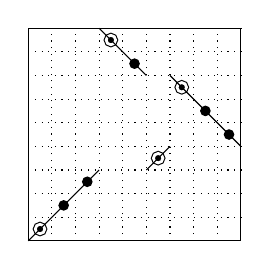
\begin{tikzpicture}[scale=.3]
	\draw (0,0) -- (9,0) -- (9,9) -- (0,9) -- cycle;
	\foreach \i in {1, 2, 3, 4, 5, 6, 7, 8, 9}{
		\draw[dotted] (0,\i) -- (9, \i);
		\draw[dotted] (\i,0) -- (\i, 9);
	}
	\draw[fill=black,double, double distance=1pt] (0.5,0.5) circle (2mm);
	\draw[fill=black] (1.5,1.5) circle (2mm);
	\draw[fill=black] (2.5,2.5) circle (2mm);
	\draw[fill=black,double, double distance=1pt] (3.5,8.5) circle (2mm);
	\draw[fill=black] (4.5,7.5) circle (2mm);
	\draw[fill=black,double, double distance=1pt] (5.5,3.5) circle (2mm);
	\draw[fill=black,double, double distance=1pt] (6.5,6.5) circle (2mm);
	\draw[fill=black] (7.5,5.5) circle (2mm);
	\draw[fill=black] (8.5,4.5) circle (2mm);

	\draw (0,0) -- (3,3);
	\draw (3,9) -- (5,7);
	\draw (5,3) -- (6,4);
	\draw (6,7) -- (9,4);

	\end{tikzpicture}
	\caption{The  wedge permutation $123984765$. Every line represents a factor, every circled point represents the leftmost element of each factor. }
	\label{fig:shape of the permutation plus factor}
\end{figure}


%\begin{remark}
%In a representation of an occurrence,
%we merge the two rightmost rectangles and replace them by the smallest rectangle that contains both of them and repeat this operation.
%Such that the right most rectangle represents the elements of the occurrence of a suffix of factor $\sigma$. See Figure \ref{fig:decomposition of an occurrence}.
%\end{remark}



\begin{figure}[t]
	\centering
	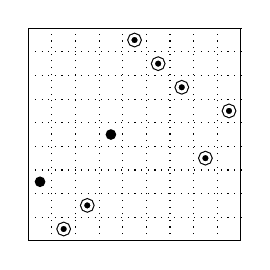
\begin{tikzpicture}[scale=.3]

	\draw (0,0) -- (9,0) -- (9,9) -- (0,9) -- cycle;
	\foreach \i in {1, 2, 3, 4, 5, 6, 7, 8, 9}{
		\draw[dotted] (0,\i) -- (9, \i);
		\draw[dotted] (\i,0) -- (\i, 9);
	}
	\draw[fill=black] (0.5,2.5) circle (2mm);
	\draw[fill=black,double, double distance=1pt] (1.5,0.5) circle (2mm);
	\draw[fill=black,double, double distance=1pt] (2.5,1.5) circle (2mm);
	\draw[fill=black] (3.5,4.5) circle (2mm);
	\draw[fill=black,double, double distance=1pt] (4.5,8.5) circle (2mm);
	\draw[fill=black,double, double distance=1pt] (5.5,7.5) circle (2mm);
	\draw[fill=black,double, double distance=1pt] (6.5,6.5) circle (2mm);
	\draw[fill=black, double distance=1pt] (7.5,3.5) circle (2mm);
	\draw[fill=black, double distance=1pt] (8.5,5.5) circle (2mm);
	\end{tikzpicture}
	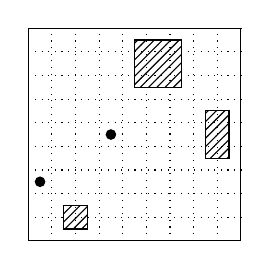
\begin{tikzpicture}[scale=.3]



	\draw (0,0) -- (9,0) -- (9,9) -- (0,9) -- cycle;
	\foreach \i in {1, 2, 3, 4, 5, 6, 7, 8, 9}{
		\draw[dotted] (0,\i) -- (9, \i);
		\draw[dotted] (\i,0) -- (\i, 9);
	}
	\draw[fill=black] (0.5,2.5) circle (2mm);
%	\draw[fill=black,double, double distance=1pt] (1.5,0.5) circle (2mm);
%	\draw[fill=black,double, double distance=1pt] (2.5,1.5) circle (2mm);
	\draw[fill=black] (3.5,4.5) circle (2mm);
%	\draw[fill=black,double, double distance=1pt] (4.5,8.5) circle (2mm);
%	\draw[fill=black,double, double distance=1pt] (5.5,7.5) circle (2mm);
%	\draw[fill=black,double, double distance=1pt] (6.5,6.5) circle (2mm);
%	\draw[fill=black, double distance=1pt] (7.5,3.5) circle (2mm);
%	\draw[fill=black, double distance=1pt] (8.5,5.5) circle (2mm);
	\draw [pattern=north east lines] (1.5,1.5) rectangle (2.5,0.5);
	\draw [pattern=north east lines] (4.5,8.5) rectangle (6.5,6.5);
	\draw [pattern=north east lines] (7.5,3.5) rectangle (8.5,5.5);

	\end{tikzpicture}
	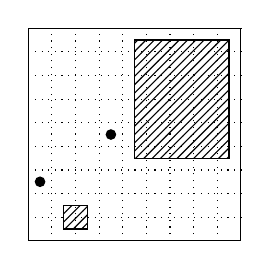
\begin{tikzpicture}[scale=.3]



	\draw (0,0) -- (9,0) -- (9,9) -- (0,9) -- cycle;
	\foreach \i in {1, 2, 3, 4, 5, 6, 7, 8, 9}{
		\draw[dotted] (0,\i) -- (9, \i);
		\draw[dotted] (\i,0) -- (\i, 9);
	}
	\draw[fill=black] (0.5,2.5) circle (2mm);
%	\draw[fill=black,double, double distance=1pt] (1.5,0.5) circle (2mm);
%	\draw[fill=black,double, double distance=1pt] (2.5,1.5) circle (2mm);
	\draw[fill=black] (3.5,4.5) circle (2mm);
%	\draw[fill=black,double, double distance=1pt] (4.5,8.5) circle (2mm);
%	\draw[fill=black,double, double distance=1pt] (5.5,7.5) circle (2mm);
%	\draw[fill=black,double, double distance=1pt] (6.5,6.5) circle (2mm);
%	\draw[fill=black, double distance=1pt] (7.5,3.5) circle (2mm);
%	\draw[fill=black, double distance=1pt] (8.5,5.5) circle (2mm);

	\draw [pattern=north east lines] (1.5,1.5) rectangle (2.5,0.5);
	\draw [pattern=north east lines] (4.5,8.5) rectangle (8.5,3.5);
	%\fill[black] (7.5,3.5) rectangle (8.5,5.5);

	\end{tikzpicture}
	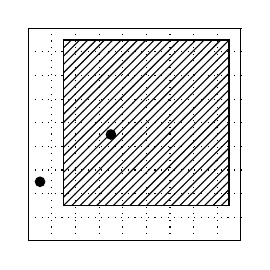
\begin{tikzpicture}[scale=.3]



	\draw (0,0) -- (9,0) -- (9,9) -- (0,9) -- cycle;
	\foreach \i in {1, 2, 3, 4, 5, 6, 7, 8, 9}{
		\draw[dotted] (0,\i) -- (9, \i);
		\draw[dotted] (\i,0) -- (\i, 9);
	}
	\draw[fill=black] (0.5,2.5) circle (2mm);
%	\draw[fill=black,double, double distance=1pt] (1.5,0.5) circle (2mm);
%	\draw[fill=black,double, double distance=1pt] (2.5,1.5) circle (2mm);
	\draw[fill=black] (3.5,4.5) circle (2mm);
%	\draw[fill=black,double, double distance=1pt] (4.5,8.5) circle (2mm);
%	\draw[fill=black,double, double distance=1pt] (5.5,7.5) circle (2mm);
%	\draw[fill=black,double, double distance=1pt] (6.5,6.5) circle (2mm);
%	\draw[fill=black, double distance=1pt] (7.5,3.5) circle (2mm);
%	\draw[fill=black, double distance=1pt] (8.5,5.5) circle (2mm);

	\draw [pattern=north east lines] (1.5,1.5) rectangle (8.5,8.5);
	%\draw [pattern=north east lines] (4.5,8.5) rectangle (8.5,3.5);
	%\fill[black] (7.5,3.5) rectangle (8.5,5.5);

	\end{tikzpicture}

	\caption{From left ro right, an occurrence of a permutation
		the same occurrence where each occurrence of a factor is represented by the minimal rectangle,
		the same occurrence where the occurrence of the first two factor are represented by the minimal rectangle
		and the same occurrence represented by its minimal rectangle.}
	\label{fig:decomposition of an occurrence}
\end{figure}




\begin{lemma}
\label{corollary:whereIsMax}
Given a wedge permutation $\sigma$,
if $\factor(i)$ is a \RLMin (resp. \RLMax) factor
the topmost (resp. bottommost) element of
$\factor(i)\ldots \factor(1)$
is the leftmost element of $\factor(i-1)$.
\end{lemma}

\begin{proof} %[of Corollary~\ref{corollary:whereIsMax}]
This corollary states that, given a wedge permutation
if the permutation starts with a \RLMin (resp. \RLMax) element then the topmost (resp. bottommost) element of this permutation is the first \RLMax (resp. \RLMin) element (see Figure \ref{fig:where to find the max}). This is easy to see from the shape of a wedge permutation.
Formally, the \RLMin elements are below the \RLMax element, thus the topmost element must be
the first \RLMax element, which is the leftmost element of $\factor(i-1)$.
\qed
\end{proof}

\begin{figure}[t]
	\centering
	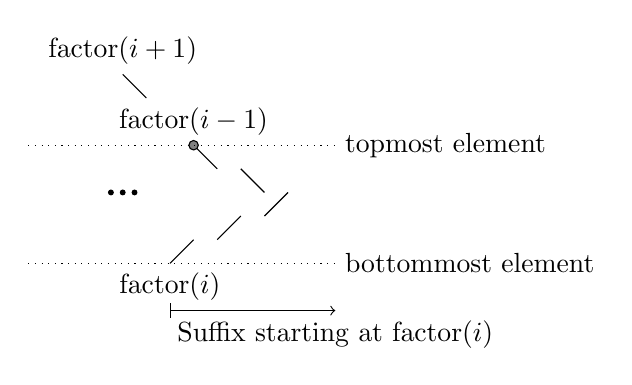
\begin{tikzpicture}[scale=.3]


%	\draw (0,0) -- (1,1);
%	\draw (2,10) -- (3,9);

	\draw[fill=black] (3.5,5) circle (1mm);
	\draw[fill=black] (4,5) circle (1mm);
	\draw[fill=black] (4.5,5) circle (1mm);

	\draw (4,10) -- (5,9);
	\draw (6,2) -- (7,3);
	\draw (7,7) -- (8,6);
	\draw (8,3) -- (9,4);
	\draw (9,6) -- (10,5);
	\draw (10,4) -- (11,5);

	\draw[fill=gray] (7,7) circle (2mm) node[above] {$\factor(i-1)$};
	\draw[fill=black] (6,2) circle (0mm) node[below] {$\factor(i)$};
		\draw[fill=black] (4,10) circle (0mm) node[above] {$\factor(i+1)$};

	\draw[dotted,-] (0,7) -- (13,7) node[right] {topmost element};
	\draw[dotted,-] (0,2) -- (13,2) node[right] {bottommost element};

	\draw[|->] (6,0) -- (13,0) node[below] {Suffix starting at $\factor(i)$};



%	\draw (6.2,2.2) -- (6.5,10);
%	\path (6.2,10) node[above] {$x$};

	\end{tikzpicture}


	\caption{
		The topmost element of the suffix starting at  $\factor(i)$
		is the leftmost element of $\factor(i-1)$ (represented by the grey dot).
		$\LM{\ppattern}{\ptext}{i}{j}$ is the smallest value of the matching of the topmost element (the grey dot) in all the occurrences of the suffix starting at $\LMEi(\factor(i))$ in $\pi[j:]$.
	}
	\label{fig:where to find the max}
\end{figure}

%We define the set
$\SET{\ppattern}{\ptext}{i}{j}$
as the set of all subsequences $s$ of $\ptext[j:]$ that start at $\ptext[j]$ and
that are  occurrences of $\factor(i)\ldots \factor(1)$.
%This set control the rectangles (not minimal) of the occurrences:
%each rectangle
%assume that $\factor(i)$ is a RLMax (resp. RLMin) factor,
%then $\pi[j]$ is the top left (resp. bottom left)
%of the rectangle of the occurrence.
%Also, note that we can always assume that the right edge
%of the rectangle is on the rightmost element of $\pi$,
%as we can always expend a rectangle of a occurrence,
%without loosing elements of the occurrence.
%We are left with the choose of the top edge,
%this is what the next lemma is for.

\begin{lemma}
\label{lemma:ts}
Let $\ppattern$ be a wedge permutation and
$\factor(i)$ be an \RLMin (resp. \RLMax) factor $\sigma$.
Let $\pi$ be a permutation and $s$ a subsequence of $\pi$ such that
$s \in \SET{\ppattern}{\ptext}{i}{j}$ and
$s$ minimizes (resp. maximizes) the matching of the leftmost element of $\factor(i-1)$.
Let $s'$ be a subsequence of $\pi$ such that
$s \in \SET{\ppattern}{\ptext}{i}{j}$
and let $t=t's'$ be a subsequence of $\pi$ that extends $s'$ on the right.
Assume $t$ is an occurrence of $\factor(i+1)\ldots \factor(1)$ such that the leftmost element of $\factor(i)$ is matched to $\ptext[j]$. Then the subsequence $t's$ is also an occurrence of $\factor(i+1)\ldots \factor(1)$ such that the leftmost element of $\factor(i)$ is matched to $\ptext[j]$.
\end{lemma}

Informally, this lemma states that we can replace
the rectangle of an occurrence in $\SET{\ppattern}{\ptext}{i}{j}$
by another rectangle of an occurrence in $\SET{\ppattern}{\ptext}{i}{j}$
such that the second rectangle shares the same edges as the first one,
except for the top edge which is lower.
Especially the second rectangle can be chosen as the one with
the lowest top edge in all the rectangles sharing the right, bottom
and left edges.
More formally, given any occurrence of $\factor(i+1)$ $\factor(i)$ $\ldots$ $\factor(1)$,
where $\factor(i)$ is a \RLMin (resp. \RLMax) factor,
we can replace the part of the occurrence where $\factor(i)$ $\ldots$ $\factor(1)$ occurs, by any occurrence
that minimises (resp. maximises) the leftmost element of $\factor(i-1)$. Indeed the leftmost element of $\factor(i-1)$ is the topmost (resp. bottommost) element of  $\factor(i)$ $\ldots$ $\factor(1)$ (see Figure \ref{fig:where to find the max}).

\begin{proof} %[of Lemma~\ref{lemma:ts}]
Let us consider the case where $\factor(i)$ is a \RLMin factor.
By definition $s$ is an occurrence of $\ppattern[\LMEi(\factor(i)):]$.
First of all, remark that $t'$ is an occurrence of $\factor(i+1)$.
So to prove that $t's$ is an occurrence of $\factor(i+1)\ldots \factor(1)$ we need to prove that the elements of t' are above the elements of $s$.
Since $t's'$ is an occurrence of $\factor(i+1)\ldots \factor(1)$ it follows that the elements of $t'$ are above the elements of $s'$. Moreover the topmost element of $s$ is below (or equal to) the topmost element of $s'$ thus the elements of $s$ are below the elements of $t'$. We use a symmetric argument if $\factor(i)$ is a \RLMax factor.
\qed
\end{proof}

\begin{corollary}
\label{corollary:we can chose a matching}
Let $\ppattern$ be a permutation,
$\factor(i)$ be a \RLMin (resp. \RLMax) factor
and
$s$ be a subsequence of $\pi$ such that $s \in \SET{\ppattern}{\ptext}{i}{j}$ and
that minimizes (resp. maximizes) the matching of the leftmost element of $\factor(i-1)$.
The following statements are equivalent:
\begin{itemize}
	\item There exists an occurrence
	 of $\ppattern$ in $\ptext$ where the leftmost element of $\factor(i)$ is matched to $\ptext[j]$.
	\item There exists an occurrence $t$ of $\factor(\ell)\ldots \factor(i+1)$ in $\ptext[:j-1]$  such that $ts$ is an occurrence of $\ppattern$ in $\ptext$ with the leftmost element of $\factor(i)$ is matched to $\ptext[j]$.
\end{itemize}
\end{corollary}

\begin{proof} %[of Corollary~\ref{corollary:we can chose a matching}]
This corollary takes a step further from the previous one, as it states that if there is no occurrence of $\ppattern$ in $\ptext$ where the leftmost element of $\factor(i)$ is matched to $\ptext[j]$ and such that
the leftmost element of $\factor(i-1)$ is minimized (resp. maximized)
then there does not exist any occurrence at all. The backward direction is trivial and the forward direction follows the Lemma~\ref{lemma:ts}.
\qed
\end{proof}

%This corollary is central to the algorithm because it allows to test only the occurrence that  minimizes (resp. maximizes) the leftmost element of $\factor(i-1)$.

%\begin{figure}[t]
%	\centering
%	\begin{tikzpicture}[scale=.3]
%
%	\draw (0,9) rectangle (3,7);
%	\draw (4,0) rectangle (6,3);
%	\draw (6,3) rectangle (12,7);
%	\draw [pattern=north east lines] (6,3) rectangle (12,6);
%
%	\end{tikzpicture}
%
%
%	\caption{In an occurrence, we can replace the rightmost rectangle by the dashed rectangle.}
%	\label{fig:minimise the max}
%\end{figure}



% This corollary allows us to way to choose a match. Indeed if one does not find a match such that a well chosen subsequence is a suffix of the pattern then there is no match at all.

\begin{proposition}
\label{Proposition:sigma avoids 213 and 231}
Let $\sigma$ be a wedge permutation of size $k$
and $\pi$ a permutation of size $n$.
One can decide in $O(max(kn^2,n^2\log(\log(n)))$ time
and $O(n^3)$ space if $\pi$ contains an occurrence $\sigma$.
\end{proposition}


\begin{proof}
The algorithm follows the previous one,
but instead of return true or false,
assuming that $\factor(i)$ is a \RLMin (resp. \RLMax) factor
the algorithm return the value of the
top (resp. bottom) edge.
So that once we compute the problem for $R_2$
we can use this value has the top (resp. bottom) edge
for the rectangle $R_1$.

We first introduce a set of values needed in the problems.
Let $LIS_{\ptext}(j,j',bound)$ (resp. $LDS_{\ptext}(j,j',bound)$) be the longest increasing
(resp. decreasing) subsequence in $\ptext[j:j']$ starting at $\pi[j]$,
with every element of this subsequence being
smaller (resp. larger) than $bound$.
$LIS_{\ptext}$ and $LDS_{\ptext}$ can be computed in
$O(n^2\log(\log(n)))$ time (see \cite{Bespamyatnikh00enumeratinglongest}).
$LIS_{\ptext}(j,j',bound)$
(resp. $LDS_{\ptext}(j,j',bound)$)
allow us to decide
the existence of an occurrence of any LRMin (resp. LRMax) factor
in the rectangle $((j,\pi[j]),(j',bound))$ (resp. $((j,bound),(j',\pi[j])$).

Given a \RLMin (resp. \RLMax) factor $\factor(i)$  of $\sigma$ and a position $j$ in $\pi$,
we want the value of the top (resp. bottom) edge
of any rectangle with left bottom (resp. with left top) corner   $(j,\pi[j])$  containing an occurrence of  $\factor(i) \ldots \factor(1)$ starting at $\pi[j]$
and which minimizes (resp. maximizes) its top (resp. bottom) edge
or a value which indicate that no occurrence exists in this rectangle. More formally:
\begin{itemize}
\item If $\factor(i)$ is \RLMin factor.

$$
\PM^\pi_\sigma(i,j) =
$$
$$
\begin{cases}

	\text{The top edge of any rectangle with left bottom corner   $(j,\pi[j])$} \\
	\text{ with right edge  $n$ containing an occurrence of  } \\
	\text{ $\factor(i) \ldots \factor(1)$ starting at $\pi[j]$ which minimize the top edge}  \\
	\text{ } \\
	\text{Or $\infty$ if no occurrence exists} \text{} \\
\end{cases}
$$

\item If $\factor(i)$ is \RLMax factor.
$$
\PM^\pi_\sigma(i,j) =
$$
$$
\begin{cases}

	\text{The bottom edge of any rectangle with left top corner   $(j,\pi[j])$} \\
	\text{ with right edge  $n$ containing an occurrence of  } \\
	\text{ $\factor(i) \ldots \factor(1)$ starting at $\pi[j]$ which
	maximize its bottom edge}  \\
	\text{ } \\
	\text{Or $0$ if no occurrence exists} \text{} \\
\end{cases}
$$

\end{itemize}

By definition, there exists an occurrence of $\ppattern$ in $\ptext$ if and only if
there exists a $1 \leq j \leq n$ such that
$\PM^\pi_\sigma(\ell,j)$ $\neq$ $0$ and $\PM^\pi_\sigma(1,\ell,j) \neq \infty$
with $\ell$ the number of factors in $\ppattern$.

We show how to compute recursively those values.
\begin{itemize}
\item If the permutation is reduced to a \RLMin (resp. \RLMax) factor
then one has to decide the top (resp. lower ) edge of
a rectangle that
contains an increasing or a decreasing factor
with the same size of larger than the
size of the unique factor starting at $\pi[j]$.
This case happens when $i=1$:

\begin{itemize}
\item If $\factor(i)$ is \RLMin factor.
$$
\PM^\pi_\sigma(1,j) = \min \text{\{$\pi[j']$ $ |$ if $ |factor(1)| \leq LIS_{\ptext}(j,j',\pi[j'])$\}}_{j'\geq j} \cup \{\infty\}
$$




\item If $\factor(i)$ is \RLMax factor.
$$
\PM^\pi_\sigma(1,j) = \min \text{\{$\pi[j']$ $ |$ if $ |factor(1)| \leq LDS_{\ptext}(j,j',\pi[j'])$\}}_{j'\geq j} \cup \{0\}
$$
\end{itemize}



\item Otherwise, if $\factor(i)$ is a \RLMin (resp. \RLMax) factor,
 we split the rectangle into two rectangles $R_1$ and
$R_2$ such that $R_1$ is left below $R_2$,
$R_1$ contains an occurrence of $\factor(i)$ starting at
$j$
and $R_2$ contains an occurrence of $\factor(i-1) \ldots factor(1)$
starting at $j'>j$.
As said before, we only need to test the pair of rectangles
where the rectangle $R_2$ has for left edge $j'$
and has the highest bottom (resp. lowest top) edge.
So for $R_2$ we want
a rectangle starting at $j'$
which contains an occurrence of $\factor(i-1) \ldots factor(i')$
starting at $j'$
with maximize the bottom (resp. minimize the top) edge.
Moreover we also want to know the value of the bottom (resp. top) edge to use it as a bound to $R_1$ so that
that $R_1$ is below $R_2$,
in other words we want $\PM^\pi_\sigma(i-1,j')$.
As before $R_1$ has to be biggest possible and
to ensure that $R_1$ is left below (resp. above) $R_2$,
$R_1$ must have for top right corner $(j'-1, \PM^\pi_\sigma(i-1,j')-1 )$
(resp. bottom right corner $(j'-1, \PM^\pi_\sigma(i-1,j')+1 )$).
Finally in all the "correct" pairs of rectangles,
we need the value of the top (resp. bottom) edge of a rectangle minimizing the top edge (resp. maximizing the bottom edge)
containing the pair of rectangles. Note that the top (resp. bottom) edge has for value $\pi[j']$
(the matching of  $\LMEi(\factor(i-1))$). Formally:

\item If $\factor(i)$ is \RLMin factor:\\
$$
\PM^\pi_\sigma(i,j) =
$$
$
\min \{\infty\} \cup \{ \pi[j'] \mid b=\PM^\pi_\sigma(i-1,j') \text{ is not $\infty$ and }
 |factor(i)| \leq LIS_{\ptext}(j,j'-1,b-1) \}_{j' < j}
$

\item If $\factor(i)$ is \RLMax factor:\\
$$
\PM^\pi_\sigma(i,j) =
$$
$
\min \{\infty\} \cup \{ \pi[j'] \mid b=\PM^\pi_\sigma(i-1,j') \text{ is not $\infty$ and }
|factor(i)| \leq LDS_{\ptext}(j,j'-1,b+1) \}_{j' < j}
$




\end{itemize}

%Informally, when deciding whether an occurrence of
%$\factor[i]\ldots \factor[1]$ starting at $j$ exists,
%assuming that $\factor(i)$ is a LRMin factor:
%We can decide whether or not the rectangle $R_1$ which has for bottom left corner
%$(j,\pi[j])$ and for top right corner $(j',bound)$
%contains an occurrence
%of $\factor[i]$, thanks to $LIS_{\ptext}(j,j',bound+1)$.
%Next we need to find an occurrence of $\factor[i-1]\ldots \factor[1]$ which is contained in a rectangle $R_2$ such that $R_2$ is right above $R_1$.
%A naive solution is to try every pair of rectangles
%resulting in a $O(n^6)$ computational time for each case.
%Indeed only the bottom left corner of $R_1$ is fixed ($(j,\pi[j])$).
%We show how to choose $R_1$ and $R_2$ in a smart way.
%\begin{itemize}
%\item The only condition requires is that $R_2$ is right above $R_1$.
%To ensure that $R_2$ is on the right of $R_1$, we fix the left edge of
%$R_2$ to $j'+1$. As said before, the right edge is the rightmost possible. Corollary~\ref{corollary:we can chose a matching} ensures that
%we only need to consider the rectangle $R_2$ with the topmost bottom edge to decide whether an occurrence exist. Moreover the value of the topmost bottom edge possible is $\LM{\ppattern}{\ptext}{i-1}{j'}$.
%So $R_2$ has for bottom edge $\LM{\ppattern}{\ptext}{i-1}{j'}$.
%\item For the top right corner of $R_1$ ($(j',bound)$),
%there is no smart way to choose $j'$, we need to iterate over
%every $j<j'$ possible. To ensure that $R_1$ is below $R_2$,
%we fix the top edge of $R_1$ to $\LM{\ppattern}{\ptext}{i-1}{j'}-1$.
%\end{itemize}
%Finally, to solve our problem,
%for every pair of rectangle which contains an occurrence of $\factor[i]\ldots \factor[1]$,
%we must find the pair, that once merged has the lowest top edge.
%The merged rectangle shares the same top edge
%as $R_2$. So we want the pair of rectangle such that
%$R_2$ has the lowest top edge.
%The case where $\factor(i)$ is a LRMax factor can be dealt with symmetry.
%More formally:
%
%
%
%\noindent\textbf{BASE:}
%\begin{align*}
%\LM{\ppattern}{\ptext}{1}{j}
%&=
%\begin{cases}
%		\min_{j<j'}\{\infty\} \cup \{\ptext[j'] |\text{ $j'$ such that \indent }
%			& \text{if $\factor(1)$ is}  \\
%		\text{ $|\factor(1)| \leq LIS(j,j',\ptext[j']+1)  $}\}
%			&\text{ a RLMin factor} \\
%		&\\
%		\max_{j<j'}\{0\} \cup \{\ptext[j'] |\text{ $j'$ such that \indent }
%			& \text{if $\factor(1)$ is}  \\
%		\text{ $|\factor(1)| \leq LDS(j,j',\ptext[j']-1) $}\}
%			&\text{ a RLMax factor}\\
%\end{cases}
%\\
%\intertext{
%In the base case,
%one is looking for an occurrence of the first factor.
%}
%\\
%\intertext{\textbf{STEP:}}
%\LM{\ppattern}{\ptext}{i}{j}
%&=
%\begin{cases}
%	\min \{\infty\} \cup  \AF{\ppattern}{\ptext}{i}{j} &
%	\text{if $\factor(i)$ is a RLMin factor}\\
%	\max \{0\} \cup  \DF{\ppattern}{\ptext}{i}{j} &
%	\text{if $\factor(i)$ is a RLMax factor}\\
%\end{cases}
%\end{align*}
%where $\AF{\ppattern}{\ptext}{i}{j}$ and $\DF{\ppattern}{\ptext}{i}{j}$ are
%the sets
%of elements matching the leftmost element of $\factor(i-1)$ in an occurrence of $\sigma[\LMEi(\factor(i)):]$ starting at $\ptext[j:]$.
%$\AF{\ppattern}{\ptext}{i}{j}$ (resp. $\DF{\ppattern}{\ptext}{i}{j}$)
%can be understand as the set of all top edges (resp. bottom edges)
%of the merged rectangles.
%$\LM{\ppattern}{\ptext}{i}{j}$  has a solution
%if and only if
%$\ptext[j:j']$ contains an occurrence of $\factor(i)$ "compatible" with an occurrence in $\ptext[j'+1:]$ of $\sigma[\LMEi(\factor(i-1)):]$. It is enough to ensure that every element of the occurrence of $\factor(i)$ is below (resp. above) the elements of the occurrence of $\sigma[\LMEi(\factor(i-1)):]$. Thus we can compute $\AF{\ppattern}{\ptext}{i}{j}$ and $\DF{\ppattern}{\ptext}{i}{j}$ as follows:
%
%\begin{align*}
%\AF{\ppattern}{\ptext}{i}{j}
%&=
%\text{$\{\ptext[j'+1] \;|\; j<j'<n$ and $\LM{\ppattern}{\ptext}{i-1}{j'+1} \neq 0$ and}
%\\
%&\qquad
%\text{$|\factor(i)| \leq LIS_{\ptext}(j,j',\LM{\ppattern}{\ptext}{i-1}{j'+1})\}$}
%\\
%\DF{\ppattern}{\ptext}{i}{j}
%&=
%\text{$\{\ptext[j'+1] \;|\; j<j'<n$ and $\LM{\ppattern}{\ptext}{i-1}{j'+1} \neq \infty$ and}
%\\
%&\qquad
%\text{$|\factor(i)| \leq LDS_{\ptext}(j,j',\LM{\ppattern}{\ptext}{i-1}{j'+1})\}$}
%\end{align*}

The number of factors is bounded by $k$.
Every instance of $LIS_{\ptext}$ and $LDS_{\ptext}$ can be computed in $O(n^2\log(\log(n))$ (see \cite{Bespamyatnikh00enumeratinglongest})
and takes $O(n^3)$ space.
There are $n$ base cases that can be computed in $O(n)$ time, thus computing every base case
takes $O(n^2)$ time.
There are $kn$ different instances of $\AFa$ and each one of them takes $O(n)$ time to compute,
thus computing every instance of $\AFa$ takes $O(kn^2)$ time.
There are $kn$ different instances of $\LMa$ and each one of them takes $O(n)$,
thus computing every $\LMa$ takes $O(kn^2)$ time.
Thus computing all the values takes $O(max(kn^2,n^2\log(\log(n)))$ time.
Every value takes $O(1)$ space, thus the problem takes $O(kn^2)$ space
but $LIS_{\ptext}$ and $LDS_{\ptext}$ takes $O(n^3)$ space.
\qed
\end{proof}

%%%%%%%%%%%%%%%%%%%%%%%%%%%%%%%%%%%%%%%%%%%%%%%%%%%%%%%%%%%%%%%%%%%%%%%%%%%%%%%

\section{Bivincular wedge permutation patterns}
	\label{section:bivincular}

This section is devoted to the pattern matching problem with bivincular wedge permutation pattern.
Recall that a bivincular pattern generalises a permutation pattern by
being able to force elements
in an occurrence
to be consecutive in value or/and in position.
%Hence,  bivincular pattern adds more restrictions on what the occurrence must look like.
%As a consequence it is easier to avoid a bivincular permutation pattern than
%the same permutation pattern.
Intuitively we cannot use the previous algorithm, as the restrictions on position and value are not managed.

Given a bivincular permutation pattern $\widetilde{\sigma}$,
we let $\widetilde{\sigma}[i:]$ refers to
the bivincular permutation pattern
which has for bottom line the bottom line of $\widetilde{\sigma}$
where we remove the elements before $i$
and has for top line the elements of $\sigma[i:]$
where $m$ and $m+1$ are overlined if and only if
$m$ and $m+1$ are in $\sigma[i:]$,
and $m$ and $m+1$ are overlined in $\widetilde{\sigma}$.
For example given $\widetilde{\sigma} = \BV{12\overline{34}\urcorner}{\llcorner 21\underline{43}}$,
$\sigma = 2143$ and
$\widetilde{\sigma}[2:] = \BV{2\overline{34}\urcorner}{1\underline{43}}$.

We describe other structures properties of wedge permutations
needed to solve the problem.

\begin{lemma}
\label{lemma:after}
Let $\sigma$ be a wedge permutation.
\begin{itemize}
\item If $\sigma[i]$ is a \RLMin element and is not the rightmost element, then $\sigma[i]+1$ is to the right of $\sigma[i]$.
\item If $\sigma[i]$ is a \RLMax element and is not the rightmost element, then $\sigma[i]-1$ is to the right of $\sigma[i]$.
\end{itemize}
\end{lemma}

\begin{proof}
For the first point,
by contradiction, $\sigma[i]+1$ would serve as a `$2$', $\sigma[i]$ would serve as a `$1$' and $\sigma[i+1]$ would serve as a `$3$' in
an occurrence of $213$.
For the second point,
by contradiction, $\sigma[i]-1$ would serve as a `$2$', $\sigma[i]$ would serve as a `$3$' and $\sigma[i+1]$ would serve as a `$1$' in
an occurrence of $231$.
\qed
\end{proof}

\begin{lemma}
\label{lemma:ascentDescentAscent}
Let $\sigma$ be a wedge permutation.
\begin{itemize}
\item If $m$ and $m+1$ are both \RLMin elements
then any element between $m$ and $m+1$ (if any)
is a \RLMax element.
\item If $m$ and $m-1$ are both RLmax elements
then any element between $m$ and $m-1$ (if any)
is a \RLMin element.
\end{itemize}

\end{lemma}


\begin{proof} %[of Lemma~\ref{lemma:ascentDescentAscent}]
For the first point, by contradiction,
let $\sigma[\alpha]=m$ and $\sigma[\beta]=m+1$
and suppose that there exists $\alpha < \gamma < \beta$,
such that $\sigma[\gamma]$ is a \RLMin element.
We know that \RLMin are strictly increasing so
$\sigma[\alpha] <  \sigma[\gamma] < \sigma[\beta]$,
which contradict the fact that $\sigma[\beta]=\sigma[\alpha]+1$.
\qed
\end{proof}

\begin{proposition}
\label{Proposition:bivincular pattern}
Let $\widetilde{\sigma}$ be a bivincular wedge permutation pattern of size $k$
and $\pi$ a permutation of size $n$.
One can decide in $O(kn^4)$ time
and $O(kn^3)$ space if $\pi$ contains an occurrence $\widetilde{\sigma}$.
\end{proposition}

\begin{proof}

%\begin{figure}[t]
%	\centering
%	\begin{tikzpicture}[scale=.3]
%	\draw[pattern=north east lines] (0,12) rectangle (1,11);
%	\draw[dotted,-] (0,10.5) -- (14,10.5) node[right] {$\ub$};
%
%	\draw[pattern=north east lines] (2,0) rectangle (3,1);
%	\draw[dotted,-] (0,1.5) -- (14,1.5) node[right] {$\lb$};
%
%	\draw[fill=black] (3,1) circle (1mm) ;
%
%	\draw[dotted,-] (3.5,12) -- (3.5,-1);
%
%	% le reste du match
%	\draw[pattern=grid] (5,8) rectangle (12,4);
%	\draw (5,4) -- (7.7,7);
%
%	%point du bot
%	\draw[fill=black] (5,4) circle (1mm) node[above] {$\pi[\ell]$} ;
%
%	\draw[thick,<->] (5,3.9) -- (5,1.5) ;
%	\draw (5,2.7) node[right] {$\overline{(\sigma[i]-1)\sigma[i]}$};
%
%	\draw[thick,<->] (4.9,4) -- (3.5,4)  node[left] {$\underline{\sigma[i-1]\sigma[i]}$};
%
%	% point du top
%	\draw[fill=black] (8,8) circle (1mm) ;
%	\draw[thick,<->] (8,8.1) -- (8,10.5) ;
%	\draw (8,9) node[right] {$\overline{\sigma[i'](\sigma[i']+1)}$};
%
%
%	\end{tikzpicture}
%	\begin{tikzpicture}[scale=.3]
%	\draw[pattern=north east lines] (0,12) rectangle (1,11);
%	\draw[dotted,-] (0,10.5) -- (14,10.5) node[right] {$\ub$};
%
%	\draw[pattern=north east lines] (2,0) rectangle (5,4);
%	\draw[dotted,-] (0,4.5) -- (14,4.5) node[right] {$\lb=\pi[\ell]+1$};
%
%	%\draw[fill=black] (3,1) circle (1mm) node[left] {$\pi[j]$};
%
%	\draw[dotted,-] (5.5,12) -- (5.5,-1);
%
%	% le reste du match
%	%\draw[dashed,red] (5,8) rectangle (12,4);
%	\draw[pattern=grid] (7,6) rectangle (12,8);
%	\draw (7,6) -- (7.7,7);
%
%
%	\draw[fill=black] (5,4) circle (1mm) ;
%
%	%point du bot
%	\draw[fill=black] (7,6) circle (1mm) node[above] {$\pi[\ell']$};
%
%
%	\draw[thick,<->] (7,5.9) -- (7,4.5) ;
%	\draw (7,5.3) node[right] {$\overline{\sigma[i]\sigma[i+1]}$};
%
%	\draw[thick,<->] (5.5,6)   node[left] {$\underline{\sigma[i]\sigma[i+1]}$} -- (6.9,6) ;
%
%	% point du top
%	\draw[fill=black] (8,8) circle (1mm) ;
%	\draw[thick,<->] (8,8.1) -- (8,10.5) ;
%	\draw (8,9) node[right] {$\overline{\sigma[i'](\sigma[i']+1)}$};
%
%
%	\end{tikzpicture}
%
%\caption{When solving $\PM{\sigma}{\ptext}{\lb}{\ub}{i}{j}$, with $\sigma[i]$ a RLMin element,
%the recursive calls of $\PM{*}{*}{*}{*}{*}{*}$ will have the same $\ub$ value,
%and the $\lb$ will be equal to the matching of $\pi[i]$ plus one. %Note that there is only ascent element before $\sigma[i']$
%}
%\label{fig:ub dont change}
%\end{figure}

Consider the following problem:
Given a lower bound $\lb$, a upper bound $\ub$, a position i of $\sigma$
and a position $j$ of $\pi$, we want to know if
there exists an occurrence of $\widetilde{\sigma}[i:]$ in $\ptext[j:]$
with every element of the occurrence is in $[\lb,\ub]$
and starting at $\pi[j]$.
In other words given the rectangle with bottom left edge
$(j,\lb)$ and with top right edge $(n,\ub)$
contains an occurrence of $\widetilde{\sigma}[i:]$
starting at $\pi[j]$,
More formally:

$$
\PM{\widetilde{\sigma}}{\ptext}{\lb}{\ub}{i}{j}=
$$
$$
\begin{cases}
	true 	& \text{if $\ptext[j:]$ has an occurrence of the bivincular pattern $\widetilde{\sigma}[i:]$ }\\
			& \text{with every element of the occurrence in $[\lb,\ub]$}\\
			& \text{and starting at $\pi[j]$}\\
			& \text{and if $\overline{\sigma[j](\sigma[j]+1)}$
			 or $\sigma[j]^\urcorner$ appear in $\widetilde{\sigma}$ then $\pi[j]=\ub$} \\
			& \text{and if $\overline{(\sigma[j]-1)\sigma[j]}$
			 or $^\ulcorner{\pi[j]}$ appear in $\widetilde{\sigma}$ then $\sigma[j]=\lb$} \\
	false 	& \text{otherwise}\\
\end{cases}
$$
Clearly if $_\llcorner{\sigma[1]}$ does not appear in $\widetilde{\sigma}$
then $\pi$ contains an occurrence of $\widetilde{\sigma}$
if and only if $\bigcup_{0<j} \PM{\widetilde{\sigma}}{\ptext}{1}{n}{1}{j}$ is true.
If $_\llcorner{\sigma[1]}$ appear in $\sigma$ then
$\pi$ contains an occurrence of
the bivincular wedge permutation pattern $\sigma$
if and only if $\PM{\widetilde{\sigma}}{\ptext}{1}{n}{1}{1}$.

We show how to compute recursively those values.
Informally, to find an occurrence of $\widetilde{\sigma}[i:]$ in $\pi[j:]$,
given that $\sigma[i]$ is a \RLMin element,
we need to find a rectangle $R$ in $\pi$
such that $R$ contains an occurrence of $\widetilde{\sigma}[i+1:]$
and $R$ is right above $\pi[j]$.
Moreover
\begin{itemize}
\item If $\underline{\sigma[i]\sigma[i+1]}$ then
we require that $\pi[j]$ and $R$ are next to each other horizontally
and that the occurrence in $R$ starts at the left edge of $R$.
In other words $R$ has for left edge $\pi[j]+1$.
\item If $\overline{\sigma[i](\sigma[i]+1)}$ then
we require that $\pi[j]$ and $R$ are next to each other vertically
and that the minimal (resp. maximal) element in the occurrence
is on the bottom (resp. top) edge of $R$.
In other words $R$ has for bottom edge $\sigma[i]+1$.
\end{itemize}
Note that the parameters $\lb$, $\ub$ and $j$ corresponding
to the occurrence of $\widetilde{\sigma}[i+1:]$ are respectively,
the bottom edge, the top edge and the left edge of the rectangle $R$.
The case where $\sigma[i]$ is a \RLMax element can be dealt with symmetry.
More formally:

\noindent\textbf{BASE:} \\
$$
\PM{\widetilde{\sigma}}{\ptext}{\lb}{\ub}{k}{j}=
\begin{cases}
	true 	& \text{if $\ptext[j] \in [\lb,\ub ]$}\\
			& \text{and if ${\ppattern[k]}_\lrcorner$ appears in $\widetilde{\sigma}$ then $j=n$}\\
			& \text{and if $_\llcorner{\sigma[k]}$ appears in $\widetilde{\sigma}$ then $j=1$}\\
			& \text{and if ${\ppattern[k]}^\urcorner$ appears in $\widetilde{\sigma}$ then $\ptext[j]=\ub=n$}\\
			& \text{and if  $^\ulcorner{\ppattern[k]}$ appears in $\widetilde{\sigma}$ then $\ptext[j]=\lb=1$ } \\
			& \text{and if  $\overline{(\ppattern[k]-1)\ppattern[k]}$ appears in $\widetilde{\sigma}$ then $\ptext[j]=\lb$ }  \\
			& \text{and if  $\overline{(\ppattern[k]\ppattern[k]+1)}$
			appears in $\widetilde{\sigma}$
			then $\ptext[j]=\ub$}  \\

	false	& \text{otherwise} \\
\end{cases}
$$

The base case finds an occurrence for the rightmost element of the pattern. If the rightmost element does not have any restriction on positions and on values, then $\PM{\sigma}{\ptext}{\lb}{\ub}{k}{j}$ is true if and only if $\ppattern[k]$ is matched to $\ptext[j]$. This is true if $\ptext[j] \in [\lb,\ub]$. If ${\ppattern[k]}_\lrcorner$ appears in $\widetilde{\sigma}$ then $\ppattern[k]$ must be matched to the rightmost element of $\pi$ thus $j$ must be $n$. If ${\ppattern[k]}^\urcorner$ appears in $\widetilde{\sigma}$ then $\ppattern[k]$ must be matched to the topmost element which is $n$. If $^\ulcorner{\ppattern[k]}$ appears in $\widetilde{\sigma}$ then $\ppattern[k]$ must be matched to the bottommost element which is $1$.
If  $\overline{(\ppattern[k]-1)\ppattern[k] }$ appears in $\widetilde{\sigma}$ then the matching element of $\ppattern[k]$ and $\ppattern[k]-1$ must be consecutive in value, by recursion the value of the element matching $\ppattern[k]-1$ will be recorded in $\lb$ and by adding $1$ to it thus $\ppattern[k]$ must be matched to $\lb$.
If  $\overline{(\ppattern[k]\ppattern[k]+1)}$ appears in $\widetilde{\sigma}$ then the element matching $\ppattern[k]$ and $\ppattern[k]+1$ must be consecutive in value, by recursion the value of the  element matching $\ppattern[k]+1$ will be recorded in $\ub$ and by removing $1$ to it thus $\ppattern[k]$ must be matched to $\ub$.

\noindent\textbf{STEP:}

In the following, we use the notation $\bigcup$ to
represent the disjunction.
We consider 3 cases for the problem $\PM{ \widetilde{\sigma}}{\ptext}{\lb}{\ub}{i}{j}$:
\begin{itemize}
	\item If $\ptext[j] \notin [\lb,\ub]$ then:
	$$
	\PM{\widetilde{\sigma}}{\ptext}{\lb}{\ub}{i}{j} = false
	$$

	which is immediate from the definition.

	\item If $\ptext[j] \in [\lb,\ub]$ and $\ppattern[i]$ is a \RLMin element then:
	$$
	\PM{\widetilde{\sigma}}{\ptext}{\lb}{\ub}{i}{j}=
	\begin{cases}
		\bigcup_{\ell>j} \PM{\widetilde{\sigma}}{\ptext}{\ptext[j]+1}{\ub}{i+1}{\ell}
			& \text{if $\ppattern[i]$ is not underlined } \\
			& \text{ and $\ppattern[i]$ is not overlined} \\
		\bigcup_{\ell>j} \PM{\widetilde{\sigma}}{\ptext}{\ptext[j]+1}{\ub}{i+1}{\ell}
			& \text{if $\ppattern[i]$ is not underlined } \\
			& \text{ and $\overline{(\ppattern[i]-1)\ppattern[i]}$ or $^\ulcorner{\ppattern[i]}$}\\
			& \text{ appears in $\widetilde{\sigma}$}\\
			& \text{ and $\ptext[j]=\lb$} \\
		\PM{\widetilde{\sigma}}{\ptext}{\ptext[j]+1}{\ub}{i+1}{j+1}
			& \text{if $\underline{\ppattern[i]\ppattern[i+1]}$ } \\
			& \text{ appears in $\widetilde{\sigma}$}\\
			& \text{ and $\ppattern[i]$ is not overlined} \\
		\PM{\widetilde{\sigma}}{\ptext}{\ptext[j]+1}{\ub}{i+1}{j+1}
			& \text{if $\underline{\ppattern[i]\ppattern[i+1]}$ } \\
			& \text{ and $\overline{(\ppattern[i]-1)\ppattern[i]}$ or $^\ulcorner{\ppattern[i]}$}\\
			& \text{ appear in $\widetilde{\sigma}$}\\
			& \text{ and $\ptext[j]=\lb$} \\
		false & \text{otherwise}

	\end{cases}
	$$
	Remark that $\ppattern[i]$  can be matched to $\pi[j]$ because $\ptext[j] \in [\lb,\ub]$.
	Thus if $\ptext[j+1:]$ has an occurrence of $\widetilde{\sigma}[i+1:]$  with every element of the occurrence in $[\pi[j]+1,\ub]$ then
 	$\ptext[j:]$ has an occurrence $\widetilde{\sigma}[i:]$.
 	To decide the latter condition,
 	it is enough to know
 	 if there exists $\ell$, $j<\ell$ such that
	$\PM{\widetilde{\sigma}}{\ptext}{\ptext[j]+1}{\ub}{i+1}{\ell}$ is true.
	The first case corresponds to an occurrence without restriction on position and on value.
	The second case asks for the matching of $\ppattern[i]-1$ and $\ppattern[i]$ to be consecutive in value, but the matching of $\ppattern[i]-1$
	is $lb-1$ thus we want $\ptext[j]=\lb$.
	The third case asks for the matching of $\ppattern[i]$ and $\ppattern[i+1]$ to be consecutive in positions, thus the matching of $\ppattern[i+1]$ must be $\pi[j+1]$.
	The fourth case is a union of the second and third case.
%	Note that we do not have to consider the case where $\overline{\ppattern[i](\ppattern[i]+1)}$ appears in $\widetilde{\sigma}$
%	as the element $(\ppattern[i]+1)$ is on the right of $\ppattern[i]$
%	(see Lemma~\ref{lemma:after})
%	and thus will
%	be taken care
%	during the calls of $\PM{\widetilde{\sigma}}{\ptext}{*}{*}{i'}{*}$
%	for some $i<i'$.
%	Identically  we do not have to consider the case
%	where $\sigma[i-1]\sigma[i]$ appears in $\widetilde{\sigma}$

	\item If $\ptext[j] \in [\lb,\ub]$ and $\ppattern[i]$ is a \RLMax element then:

	$$
	\PM{\widetilde{\sigma}}{\ptext}{\lb}{\ub}{i}{j}=
	\begin{cases}
			\bigcup_{\ell>j} \PM{\widetilde{\sigma}}{\ptext}{\lb}{\ptext[j]-1}{i+1}{\ell}
				& \text{if $\ppattern[i]$ is not underlined } \\
				& \text{ and $\ppattern[i]$ is not overlined} \\
			\bigcup_{\ell>j} \PM{\widetilde{\sigma}}{\ptext}{\lb}{\ptext[j]-1}{i+1}{\ell}
				& \text{if $\ppattern[i]$ is not underlined } \\
				& \text{ and $\overline{\ppattern[i](\ppattern[i]+1)}$ or ${\ppattern[i]}^\urcorner$}\\
				& \text{ appear in $\widetilde{\sigma}$}\\
				& \text{ and $\ptext[j]=\ub$} \\
			\PM{\widetilde{\sigma}}{\ptext}{\lb}{\ptext[j]-1}{i+1}{j+1}
				& \text{if $\underline{\ppattern[i]\ppattern[i+1]}$ } \\
				& \text{ appears in $\widetilde{\sigma}$}\\
				& \text{ and $\ppattern[i]$ is not overlined} \\
			\PM{\widetilde{\sigma}}{\ptext}{\lb}{\ptext[j]-1}{i+1}{j+1}
				& \text{if $\underline{\ppattern[i]\ppattern[i+1]}$ } \\
				& \text{ and $\overline{\ppattern[i](\ppattern[i]+1)}$ or ${\ppattern[i]}^\urcorner$}\\
				& \text{ appear in $\widetilde{\sigma}$}\\
				& \text{ and $\ptext[j]=\ub$} \\
			false & \text{otherwise}
	\end{cases}
	$$
	The same remark as the last case holds.
\end{itemize}

Remark that there are constraints that we do not concern given in
$\PM{\widetilde{\sigma}}{\ptext}{*}{*}{i}{*}$.
Especially in the case where $\sigma[i]$ is a \RLMin
the case where $\underline{\sigma[i-1]\sigma[i]}$,
$\overline{\ppattern[i](\ppattern[i]+1)}$
and every combination of the constraints
appear in $\widetilde{\sigma}$
are not in the conditions.
$\underline{\sigma[i-1]\sigma[i]}$ is not
in the conditions because it is
up to $\PM{\widetilde{\sigma}}{\ptext}{*}{*}{i-1}{*}$
to ensure that the elements corresponding to elements at position $i-1$ and $i$ in an occurrence are next to each other in position.
$\overline{\ppattern[i](\ppattern[i]+1)}$ is not
in the conditions because $\sigma[i]+1$ is on the right
of $\sigma[i]$ (see Lemma~\ref{lemma:after})
and thus will
be taken care
during the calls of $\PM{\widetilde{\sigma}}{\ptext}{*}{*}{i'}{*}$
for some $i<i'$.
In the same fashion,
when $\sigma[i]$ is a \RLMax $\underline{\sigma[i-1]\sigma[i]}$
do not appear in the conditions for the exact same reason
and $\overline{(\ppattern[i]-1)\ppattern[i]}$
because $\sigma[i]-1$ is on the right of $\sigma[i]$.

Clearly the problem return true if $\pi$ contains an
occurrence of $\widetilde{\sigma}$ if there is no constraint on position
and on value.
We now discus how the position and value constraints
are taken into account so that the algorithm
returns true if and only if $\pi$ has an occurrence
of $\widetilde{\sigma}$.

\paragraph{Position Constraint.} There are 3 types of position constraints that can be added by underlined elements.
\begin{itemize}
	\item If $_\llcorner{\sigma[1]}$ appears in $\widetilde{\sigma}$ then the leftmost element of $\sigma$  must be matched to the leftmost element of $\pi$ ($\ppattern[1]$ is matched to $\ptext[1]$ in a occurrence of $\ppattern$ in $\ptext$). This constraint is satisfied by requiring that the occurrence starts at the leftmost element of $\ptext$: if  $\PM{\widetilde{\sigma}}{\ptext}{1}{n}{1}{1}$ is true.

	\item If ${\ppattern[k]}_\lrcorner$ appears in $\widetilde{\sigma}$ then the rightmost element $\sigma$ must be matched the rightmost element of $\pi$ ($\ppattern[k]$ is matched to $\ptext[n]$ on a occurrence of $\ppattern$ in $\ptext$). This constraint is checked in the base case.

	\item If $\underline{\ppattern[i]\ppattern[i+1]}$ appears in $\widetilde{\sigma}$ then the positions of the element matching $\ppattern[i]$ and $\ppattern[i+1]$ must be consecutive. In other words, if $\ppattern[i]$ is matched to $\ptext[j]$ then $\ppattern[i+1]$ must be matched to $\ptext[j+1]$. We ensure this restriction by recursion by requiring that the matching of $\ppattern[i+1:]$ starts at position $j+1$.
\end{itemize}

\paragraph{Value Constraint.} There are 3 types of value constraints that can be added by overlined elements.
\begin{itemize}
	\item If $^\ulcorner{\sigma[i]}$ appears in $\widetilde{\sigma}$ (and thus $\sigma[i]=1$) then the bottommost element of $\ppattern$ must be matched to the bottommost element of $\ptext$.
	\begin{itemize}

		\item If $\sigma[i]$ is a \RLMin element, then remark that:
		\begin{itemize}
			\item Every problem
			$\PM{\widetilde{\sigma}}{\ptext}{\lb}{*}{i}{*}$ is true only if $\sigma[i]$ is matched to the element with value $\lb$ (by recursion).
			So it is enough to require that $\lb=1$.
			\item The recursive calls for $\sigma[1]$, $\ldots$, $\sigma[i-1]$
			do not change the lower bound as
			$\sigma[i]$ is the leftmost \RLMin element. Indeed if not, then there exists a \RLMin element $\sigma[i']$, $i'<i$ and by the shape of a wedge permutation $\sigma[i']<\sigma[i]$ which is not possible as $\sigma[i]$ must be the bottommost element.
			As a consequence $\sigma[1]$, $\ldots$, $\sigma[i-1]$ are \RLMax elements. Finally the recursive calls for \RLMax elements do not change the lower bound.
			\item The first call of the problem has for parameter $\lb=1$.
		\end{itemize}
		So $\PM{\widetilde{\sigma}}{\ptext}{*}{*}{i}{*}$ return true only if
		$\sigma[i]$ is matched to $1$.

		\item If $\sigma[i]$ is a \RLMax element then $i=k$ ($\sigma[i]$ is the rightmost element). Thus every $\PM{\widetilde{\sigma}}{\ptext}{*}{*}{i}{*}$ is a base case and is true only if $\sigma[i]$ is matched to $1$.

	\end{itemize}




	\item If ${\ppattern[i]}^\urcorner$ appears in $\widetilde{\sigma}$ (and thus $\sigma[i]=k$) then the topmost element of $\ppattern$ must be matched to the topmost element of $\ptext$.
	\begin{itemize}

		\item If $\sigma[i]$ is a \RLMax element, then remark that:
		\begin{itemize}
			\item Every problem
			$\PM{\widetilde{\sigma}}{\ptext}{*}{\ub}{i}{*}$ is true only if $\sigma[i]$ is matched to the element with value $\ub$ (by recursion).
			So it is enough to require that $\ub=n$.
			\item The recursive calls for $\sigma[1]$, $\ldots$, $\sigma[i-1]$
			do not change the upper bound as
			$\sigma[i]$ is the leftmost \RLMax element. Indeed if not, then there exists a \RLMax element $\sigma[i']$, $i'<i$ and by the shape of a wedge permutation $\sigma[i']>\sigma[i]$ which is not possible as $\sigma[i]$ must be the topmost element.
			As a consequence $\sigma[1]$, $\ldots$, $\sigma[i-1]$ are \RLMin elements. Finally the recursive calls for \RLMin elements do not change the upper bound.
			\item The first call of the problem has for parameter $\ub=n$.
		\end{itemize}
		So $\PM{\widetilde{\sigma}}{\ptext}{*}{*}{i}{*}$ return true only if
		$\sigma[i]$ is matched to $n$.

		\item If $\sigma[i]$ is a \RLMin element then $i=k$ ($\sigma[i]$ is the rightmost element). Thus every $\PM{\widetilde{\sigma}}{\ptext}{*}{*}{i}{*}$ is a base case and is true if $\sigma[i]$ is matched to $n$.

	\end{itemize}



	\item  If $\overline{\ppattern[i]\ppattern[i']}$ appears in $\widetilde{\sigma}$,  (which implies that $\ppattern[i']=\ppattern[i]+1$) then if $\ppattern[i]$ is matched to $\ptext[j]$ then $\ppattern[i']$ must be matched to $\ptext[j]+1$
	or f $\ppattern[i']$ is matched to $\ptext[j]$ then $\ppattern[i]$ must be matched to $\ptext[j]-1$.

		\begin{itemize}

			\item The cases $\ppattern[i]$ is a \RLMax element, $\ppattern[i']$ is a \RLMin element and $i<i'$ or  $\ppattern[i]$ is a \RLMin element, $\ppattern[i']$ is a \RLMax element and $i'<i$ are not possible.
			Indeed $\ppattern[i]$ is the topmost element of $\ppattern[i:]$ thus $\ppattern[i] > \ppattern[i']$ which is in contradiction with
			$\ppattern[i']=\ppattern[i]+1$.

			\item If $\ppattern[i]$ is a \RLMin element, $\ppattern[i']$ is a \RLMax element and $i<i'$ (remark that this case is symmetric to the case where $\ppattern[i]$ is a \RLMax element, $\ppattern[i']$ is a \RLMin element and $i'<i$), then
			remark that
			\begin{itemize}
				\item $i'=k$, indeed if $i'$ is not the right most element, there would exist an element between
				$\sigma[i]$ and $\sigma[i']$. So every recursive call
				$\PM{\widetilde{\sigma}}{\ptext}{\lb}{*}{i'}{*}$
				is solved as a base case. So $\PM{\widetilde{\sigma}}{\ptext}{\lb}{*}{i'}{*}$ is true only if $\sigma[i']$ is matched to the element with $\lb$.
				\item The recursive calls for $\sigma[i+1]$, $\ldots$, $\sigma[i'-1]$ do not change the lower bound.
				Indeed $\ppattern[i]$ is the rightmost \RLMin.
				So $\sigma[i+1]$, $\sigma[i+2]$, $\ldots$, $\sigma[i'-1]$ are \RLMax elements. Moreover
				recursive calls for a \RLMax do not change the lower bound.
				\item $\PM{\widetilde{\sigma}}{\ptext}{\lb}{*}{i}{*}$ sets
				the $\lb$ to $\ptext[j]+1$ and matches $\sigma[i]$ to $\ptext[j]$.
			\end{itemize}
			So $\sigma[i]$ is matched to $\ptext[j]$ and
			$\sigma[i']$ is matched to $\ptext[j]+1$.

			\item If $\ppattern[i]$ is a \RLMin element and $\ppattern[i']$ is a \RLMin element then
			first remark:
			\begin{itemize}

				\item From lemma~\ref{lemma:ascentDescentAscent},
				we have that $i<i'$.

				\item  Every recursive call $\PM{\widetilde{\sigma}}{\ptext}{\lb}{*}{i'}{*}$ is true only if $\sigma[i']$ is matched to the element with value $\lb$.

				\item  The recursive calls for $\sigma[i+1]$, $\ldots$, $\sigma[i'-1]$ do not change the lower bound. Indeed
				from lemma~\ref{lemma:ascentDescentAscent}, $\sigma[i+1]$,  $\ldots$, $\sigma[i'-1]$ are \RLMax elements. Finally the recursive calls for \RLMax elements do not change the lower bound.

				\item $\PM{\widetilde{\sigma}}{\ptext}{*}{*}{i}{*}$ sets $\lb$ to $\ptext[j]+1$ and matches $\sigma[i]$ to $\ptext[j]$.

			\end{itemize}
			So $\sigma[i]$ is matched to $\ptext[j]$ and
			$\sigma[i']$ is matched to $\ptext[j]+1$.


			\item If $\ppattern[i]$ is a \RLMax element and $\ppattern[i']$ is a \RLMax element then
			first remark:
			\begin{itemize}
				\item From lemma~\ref{lemma:ascentDescentAscent},
				we have that $i'<i$.

				\item  Every recursive call $\PM{\widetilde{\sigma}}{\ptext}{*}{\ub}{i}{*}$ is true only if $\sigma[i]$ is matched to the element with value $\ub$.

				\item  The recursive calls for $\sigma[i+1]$, $\ldots$, $\sigma[i'-1]$ do not change the upper bound. Indeed
				from lemma~\ref{lemma:ascentDescentAscent}, $\sigma[i+1]$,  $\ldots$, $\sigma[i'-1]$ are \RLMin elements. Finally the recursive calls for \RLMin elements do not change the upper bound.

				\item $\PM{\widetilde{\sigma}}{\ptext}{*}{*}{i'}{*}$ sets $\ub$ to $\ptext[j]-1$ and matches $\sigma[i']$ to $\ptext[j]$.

			\end{itemize}
			So $\sigma[i']$ is matched to $\ptext[j]$ and
			$\sigma[i]$ is matched to $\ptext[j]-1$.


		\end{itemize}
\end{itemize}

There are $n^3$ base cases that can be computed in constant time.
There are $kn^3$ different cases. Each case takes up to $O(n)$ time to compute.
Thus computing all the cases take $O(kn^4)$ time.
Each case take $O(1)$ space, thus we need $O(kn^3)$ space.
\qed
\end{proof}

%%%%%%%%%%%%%%%%%%%%%%%%%%%%%%%%%%%%%%%%%%%%%%%%%%%%%%%%%%%%%%%%%%%%%%%%%%%%%%%

\section{Computing the longest wedge permutation pattern}
\label{section:LCS}

This section is focused on a problem related to the permutation pattern matching problem.
Given a set of permutations, one must compute the longest permutation
which occurs in each permutation in the set.
This problem is known to be NP-Hard for an arbitrary size of the set even
when all the permutations of this set are separable permutations (See~\cite{2007math......2109B}).
We show how to compute the longest wedge permutation
occurring in a set.
We do not hope that this problem is solvable in polynomial time
if the size of the set is not fixed.
Indeed the size of the set appears in the exponent
in the complexity of the algorithm.
Thus we focus on the cases where only one or two permutations are given in set.

Conveniently, we say that a subsequence is
a wedge subsequence if and only if the permutation represented by the subsequence
is a wedge permutation.

We start with the easiest case where we are given just one input permutation.
We need the set of \RLMax elements and the set of \RLMin elements.
$A(\pi) = \{i | \text{$\pi[i]$ is a \RLMin element} \} \cup \{n\}$ and
$D(\pi) = \{i | \text{$\pi[i]$ is a \RLMax element} \} \cup \{n\}$.\\


\begin{proposition}
\label{proposition:longestIncreasingSubsequence}
If $s_i$ is the longest increasing subsequence with last element at position $f$ in $\pi$
and $s_d$ is the longest decreasing subsequence with last element at position $f$ in $\pi$
then $s_i \cup s_d$ is a longest wedge subsequence with last element at position $f$ in $\pi$.
\end{proposition}

\begin{proof}
Let us first prove that we have a wedge subsequence.
$s_i$ is an increasing subsequence with values below or equal $\pi[f]$ and
$s_d$ is an decreasing subsequence with values above or equal $\pi[f]$,
so $s_i \cup s_d$ is a wedge subsequence.
Let us prove that this is a longest.
Let $s$ be a wedge subsequence with its rightmost element at position $f$ in $\pi$ such
that $|s|>|s_i \cup s_d|$,
first note that $A(s)$ is also an increasing subsequence with its rightmost  at position $f$ in $\pi$
and $D(s)$ is also an decreasing subsequence with its rightmost  at position $f$ in $\pi$,
then as $|s|>|s_i \cup s_d|$ then either $|A(s)| > |s_i|$ or $|D(s)| > |s_d|$,
which is in contradiction with the definition of $s_i$ and $s_d$.
\end{proof}

%\begin{proposition}
%\label{proposition:longestIncreasingSubsequence}
%If $s$ is an occurrence of a  longest $(213,231)$-avoiding subsequence with last element at position
%$f$ in $\pi$ then
%$A(s)$ is a longest increasing subsequence with last element at position $f$ and
%$D(s)$ is a longest decreasing subsequence with last element at position $f$.
%\end{proposition}
%
%\begin{proof}[of Proposition~\ref{proposition:longestIncreasingSubsequence}]
%Let $s$ be a longest subsequence avoiding (213,231) with last element at position $f$ in $\pi$,
%suppose that $A(s)$ is not a longest increasing subsequence with last element at position $f$. Let $s_m$ be a longest increasing subsequence with last element $f$.
%Thus $|s_m|>|A(s)|$, clearly the sequence $s_m \cup D(s)$ is longer than $s$.
%Moreover the sequence $s_m \cup D(s)$ avoid both $213$ and $231$ as  $s_m$ is an increasing
%subsequence with value lower and equal than $\pi[f]$ and $D(s)$ is an decreasing subsequence
%with value above or equal than $\pi[f]$.
%In other words $s$ is not the longest subsequence avoiding (213,231) with last element at position $f$ in $\pi$. Which is a contradiction.
%The same idea can be used to show that $D(\pi)$ is the longest decreasing subsequence.
%\qed
%\end{proof}

\begin{proposition}
\label{proposition:longest 2}
Let $\pi$ be a permutation. One can compute
the longest wedge subsequence that can occur in $\pi$
in $O(n\log(\log(n)))$ time and in $O(n)$ space.
\end{proposition}

\begin{proof}[of Proposition~\ref{proposition:longest 2}]
Proposition \ref{proposition:longestIncreasingSubsequence} leads to an algorithm
where one computes the longest increasing and decreasing subsequence ending at every  possible position
and then finds the maximum sum of longest increasing and decreasing subsequence ending at the same position.
Computing the longest increasing subsequences and the longest decreasing subsequences can be done in
$O(n\log(\log(n)))$ time and $O(n)$ space
(see \cite{Bespamyatnikh00enumeratinglongest}),
then finding the maximum can be done in linear time.
\qed
\end{proof}

We  now consider the case where the input is composed of two permutations.


\begin{proposition}
Given two permutations $\pi_1$ of size $n_1$ and $\pi_2$ of size $n_2$,
one can compute
the longest common wedge subsequence
in $O(n_1^3n_2^3)$ time and space.
\end{proposition}

\begin{proof}
Consider the following problem
that computes the longest wedge subsequence common to $\pi_1$ and $\pi_2$:
Given two permutations $\pi_1$ and $\pi_2$, we define
$
\LCS{\pi_1}{\lb_1}{\ub_1}{\pi_2}{\lb_2}{\ub_2}{i_1}{i_2}
$
\begin{center}
= $\max$ \{$|s|$ $|$ $s$ occurs $\pi_1[i_1:]$ with every element of the occurrence in $[\lb_1,\ub_1]$ and $s$ occurs $\pi_2[i_2:]$ with every element of the occurrence in $[\lb_2,\ub_2]$ and $s$ is a wedge subsequence
 \}
\end{center}



We show how to solve this problem by dynamic programming.

\noindent\textbf{BASE:}
$$
\LCS{\pi_1}{\lb_1}{\ub_1}{\pi_2}{\lb_2}{\ub_2}{n_1}{n_2} =
\begin{cases}
	1 & \text{if $\lb_1 \leq \pi_1[n_1] \leq \ub_1$
	}\\
	& \text{ and $\lb_2 \leq \pi_2[n_2] \leq \ub_2$}\\
	0 & \text{otherwise}\\
\end{cases}
$$

\noindent\textbf{STEP:}
$$
\LCS{\pi_1}{\lb_1}{\ub_1}{\pi_2}{\lb_2}{\ub_2}{i_1}{i_2}=\max
\begin{cases}
	\LCS{\pi_1}{\lb_1}{\ub_1}{\pi_2}{\lb_2}{\ub_2}{i_1}{i_2+1} \\
	\\
	\LCS{\pi_1}{\lb_1}{\ub_1}{\pi_2}{\lb_2}{\ub_2}{i_1+1}{i_2} \\
	\\
	\match{\pi_1}{\lb_1}{\ub_1}{\pi_2}{\lb_2}{\ub_2}{i_1}{i_2}
\end{cases}
$$

with \\
$
\match{\pi_1}{\lb_1}{\ub_1}{\pi_2}{\lb_2}{\ub_2}{i_1}{i_2}=
\begin{cases}
1+\LCS{\pi_1}{\pi_1[i_1]+1}{\ub_1}{\pi_2}{\pi_2[i_2]+1}{\ub_2}{i_1+1}{i_2+1}
	& \text{$\pi_1[i_1]<\lb_1$ } \\
	& \text{and $\pi_2[i_2]<\lb_2$} \\

&\\

1+\LCS{\pi_1}{\lb_1}{\pi_1[i_1]-1}{\pi_2}{\lb_2}{\pi_2[i_2]-1}{i_1+1}{i_2+1}
	& \text{$\pi_1[i_1]>\ub_1$ } \\
	&\text{and $\pi_2[i_2]>\ub_2$}\\

&\\

0 	& \text{otherwise}\\
\end{cases}
$

%For every pair $i,j$ we either ignore the element of $\pi_1$,
%or we ignore the element of $\pi_2$,
%or we match as the same step (if possible).

The solution to the problem relies on the fact
that the longest wedge subsequence is found
either by considering the problem with $\pi_1[i_1:]$ and $\pi_2[i_2+1:]$
or by considering the problem with $\pi_1[i_1+1:]$ and $\pi_2[i_2:]$
or by matching  $\pi_1[i_1]$ and $\pi_2[i_2]$ and adding
to the solution the LCS for $\pi_1[i_1+1:]$ and $\pi_2[i_2+1:]$ which is compatible,
meaning that if we consider the current elements
to correspond to a \RLMin (resp. \RLMax) element in the longest wedge subsequence
then we consider only the solution with elements above (below)
$\pi_1[i_1]$ for the occurrence in $\pi_1[i_1+1:]$
and $\pi_2[i_2]$ for the occurrence in $\pi_2[i_2+1:]$.

These relations lead to a $O(|\pi_1|^3|\pi_2|^3)$ time and $O(|\pi_1|^3|\pi_2|^3)$ space algorithm.
Indeed there are $|\pi_1|^3|\pi_2|^3$  possible cases for the problem
and each case is solved in constant time.
$\qed$
\end{proof}


\bibliography{bibli}{}
\bibliographystyle{plain}


%%%%%%%%%%%%%%%%%%%%%%%%%%%%%%%%%%%%%%%%%%%%%%%%%%%%%%%%%%%%%%%%%%%%%%%%%%%%%%%


\end{document}
